\section{2022年高考题}

\subsection{2022年全国甲卷（理）}\label{gk:2022年全国甲卷（理）}

\begin{description}
    \item[一、选择题] 本题共12小题，每小题5分，共60分．在每小题给出的四个选项中，只有一项是符合题目要求的．
    \begin{enumerate}[leftmargin=5pt]
        \item 若 $z=-1+\sqrt{3}\i$，则 $\dfrac{z}{z\bar{z}-1}=$
       
        {\centering\begin{tabular*}{\linewidth}{@{}@{\extracolsep{\fill}}llll@{}}
          \(\text{A. }-1+\sqrt{3}\i\)  & \(\text{B. }-1-\sqrt{3}\i\)  & \(\text{C. }-\dfrac{1}{3}+\dfrac{\sqrt{3}}{3}\i\)  & \(\text{D. }-\dfrac{1}{3}-\dfrac{\sqrt{3}}{3}\i\)
        \end{tabular*}\par}

        \item 某社区通过公益讲座以普及社区居民的垃圾分类知识．为了解讲座效果，随机抽取10位社区居民，让他们在讲座前和讲座后各回答一份垃圾分类知识问卷，这10位社区居民在讲座前和讲座后问卷答题的正确率如下图：
        
        {\centering
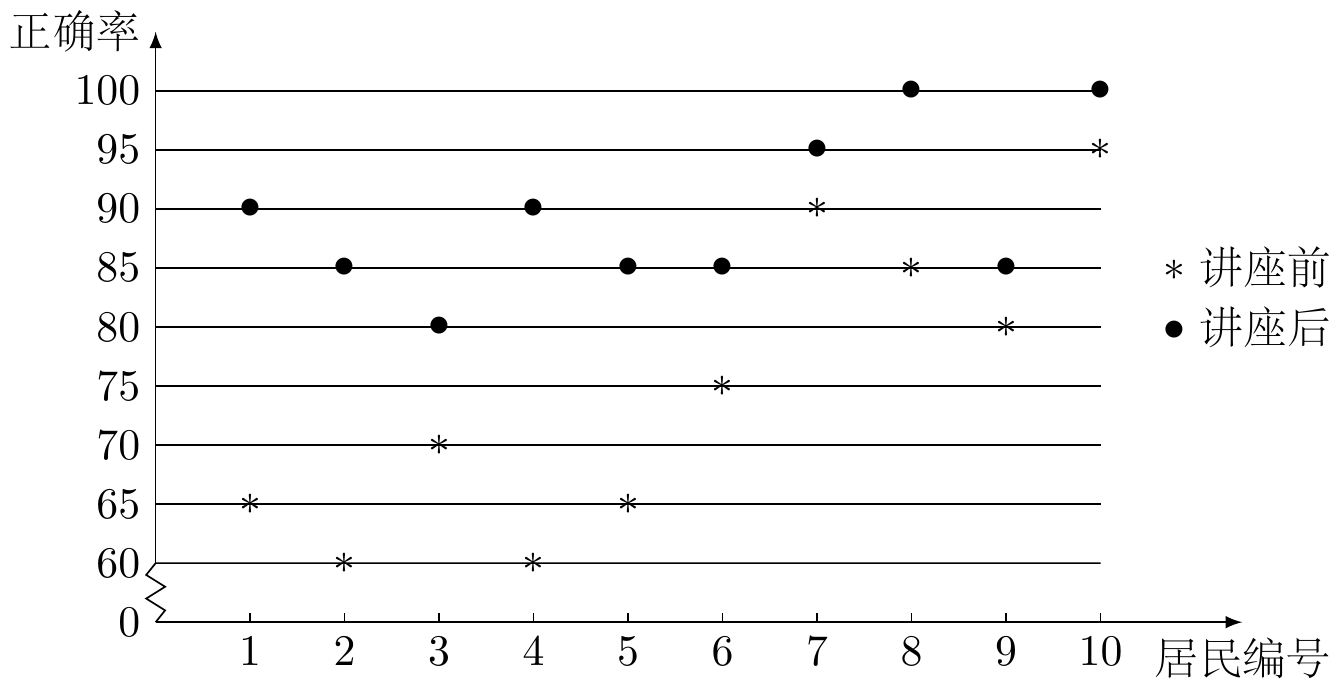
\includegraphics[width=13.0cm]{GaoKao/images/2022/national_paper_a_science/q2_fig1.png}
\par}

        则
       
        {\centering\begin{tabular*}{\linewidth}{@{}@{\extracolsep{\fill}}llll@{}}
          \(\text{A. }\)讲座前问卷答题的正确率的中位数小于$70\%$ \\
          \(\text{B. }\)讲座后问卷答题的正确率的平均数大于$85\%$ \\
          \(\text{C. }\)讲座前问卷答题的正确率的标准差小于讲座后正确率的标准差 \\
          \(\text{D. }\)讲座后问卷答题的正确率的极差大于讲座前正确率的极差
        \end{tabular*}\par}

        \item 设全集 $U=\{-2,-1,0,1,2,3\}$，集合 $A=\{-1,2\}$，$B=\{x\mid x^2-4x+3=0\}$，则 $\complement_U(A\cup B)=$
       
        {\centering\begin{tabular*}{\linewidth}{@{}@{\extracolsep{\fill}}llll@{}}
          \(\text{A. }\{1,3\}\)  & \(\text{B. }\{0,3\}\)  & \(\text{C. }\{-2,1\}\)  & \(\text{D. }\{-2,0\}\)
        \end{tabular*}\par}

        \item 如图，网格纸上绘制的是一个多面体的三视图，网格小正方形的边长为1，则该多面体的体积为
        
        {\centering
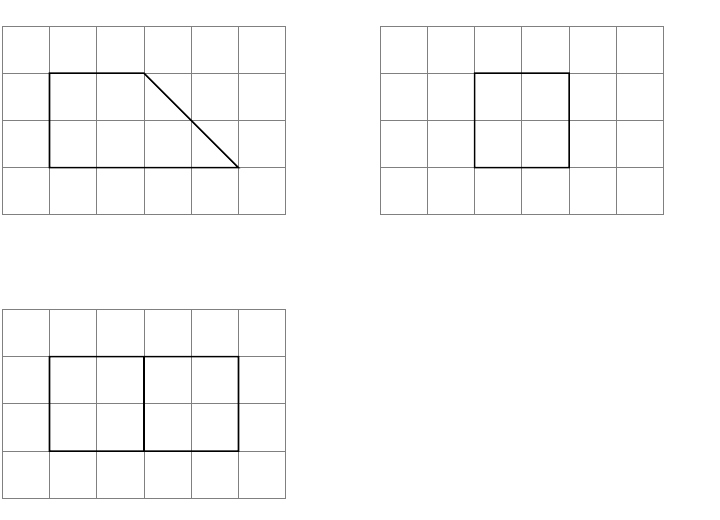
\includegraphics[width=7.0cm]{GaoKao/images/2022/national_paper_a_science/q4_fig1.png}
\par}

        {\centering\begin{tabular*}{\linewidth}{@{}@{\extracolsep{\fill}}llll@{}}
          \(\text{A. }8\)  & \(\text{B. }12\)  & \(\text{C. }16\)  & \(\text{D. }20\)
        \end{tabular*}\par}

        \item 函数 $y=(3^x-3^{-x})\cos x$ 在区间 $\bigl[-\frac{\pi}{2},\frac{\pi}{2}\bigr]$ 的图象大致为
        
        {\centering
            \begin{tabular*}{\linewidth}{@{}@{\extracolsep{\fill}}cccc@{}}
            \(\text{A. }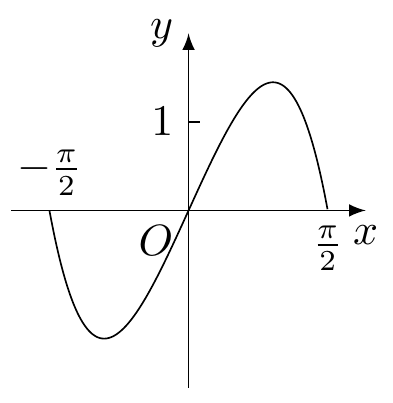
\includegraphics[width=0.15\paperwidth]{GaoKao/images/2022/national_paper_a_science/q5_optA.png}\)  &  \(\text{B. }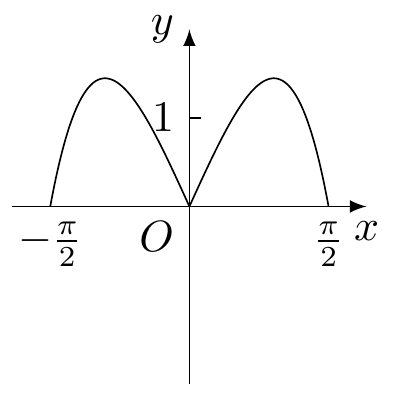
\includegraphics[width=0.15\paperwidth]{GaoKao/images/2022/national_paper_a_science/q5_optB.png}\)  &  \(\text{C. }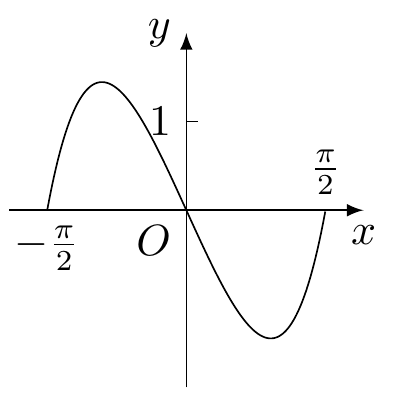
\includegraphics[width=0.15\paperwidth]{GaoKao/images/2022/national_paper_a_science/q5_optC.png}\)  &  \(\text{D. }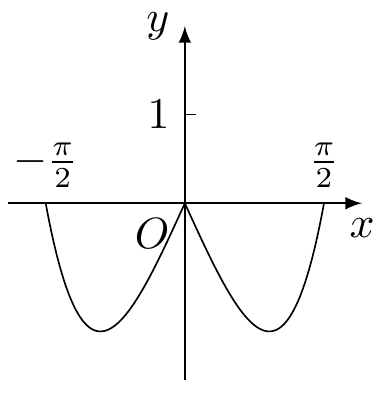
\includegraphics[width=0.15\paperwidth]{GaoKao/images/2022/national_paper_a_science/q5_optD.png}\)
        \end{tabular*}
        \par}

        \item 当 $x=1$ 时，函数 $f(x)=a\ln x+\dfrac{b}{x}$ 取得最大值 $-2$，则 $f'(2)=$
       
        {\centering\begin{tabular*}{\linewidth}{@{}@{\extracolsep{\fill}}llll@{}}
          \(\text{A. }-1\)  & \(\text{B. }-\dfrac{1}{2}\)  & \(\text{C. }\dfrac{1}{2}\)  & \(\text{D. }1\)
        \end{tabular*}\par}

        \item 在长方体 $ABCD$-$A_1B_1C_1D_1$ 中，已知 $B_1D$ 与平面 $ABCD$ 和平面 $AA_1B_1B$ 所成的角均为 $30^\circ$，则
       
        {\centering\begin{tabular*}{\linewidth}{@{}@{\extracolsep{\fill}}llll@{}}
          \(\text{A. }AB=2AD\)  & \(\text{B. }AB$ 与平面 $AB_1C_1D$ 所成的角为 $30^\circ$ \\
          \(\text{C. }AC=CB_1\)  & \(\text{D. }B_1D$ 与平面 $BB_1C_1C$ 所成的角为 $45^\circ\)
        \end{tabular*}\par}

        \item 沈括的《梦溪笔谈》是中国古代科技史上的杰作，其中收录了计算圆弧长度的"会圆术"．如图，$$\widehat{AB}$$ 是以 $O$ 为圆心，$OA$ 为半径的圆弧，$C$ 是 $AB$ 的中点，$D$ 在 $$\widehat{AB}$$ 上，$CD\perp AB$．"会圆术"给出 $$\widehat{AB}$$ 的弧长的近似值 $s$ 的计算公式：$s=AB+\dfrac{CD^2}{OA}$．当 $OA=2$，$\angle AOB=60^\circ$ 时，$s=$
        
        {\centering
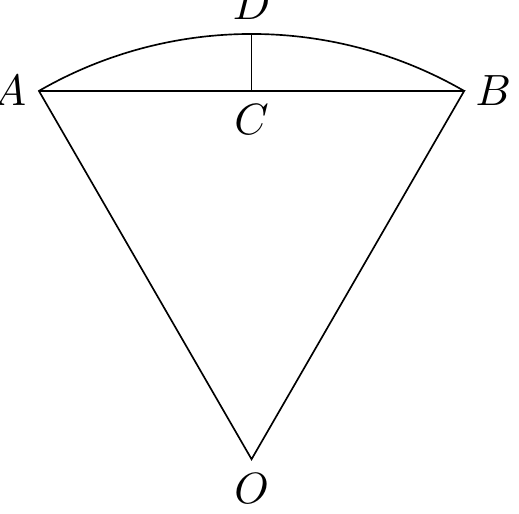
\includegraphics[width=2.7cm]{GaoKao/images/2022/national_paper_a_science/q8_fig1.png}
\par}

        {\centering\begin{tabular*}{\linewidth}{@{}@{\extracolsep{\fill}}llll@{}}
          \(\text{A. }\dfrac{11-3\sqrt{3}}{2}\)  & \(\text{B. }\dfrac{11-4\sqrt{3}}{2}\)  & \(\text{C. }\dfrac{9-3\sqrt{3}}{2}\)  & \(\text{D. }\dfrac{9-4\sqrt{3}}{2}\)
        \end{tabular*}\par}

        \item 甲、乙两个圆锥的母线长相等，侧面展开图的圆心角之和为 $2\pi$，侧面积分别为 $S_{\text{甲}}$ 和 $S_{\text{乙}}$，体积分别为 $V_{\text{甲}}$ 和 $V_{\text{乙}}$．若 $\dfrac{S_{\text{甲}}}{S_{\text{乙}}}=2$，则 $\dfrac{V_{\text{甲}}}{V_{\text{乙}}}=$
       
        {\centering\begin{tabular*}{\linewidth}{@{}@{\extracolsep{\fill}}llll@{}}
          \(\text{A. }\sqrt{5}\)  & \(\text{B. }2\sqrt{2}\)  & \(\text{C. }\sqrt{10}\)  & \(\text{D. }\dfrac{5\sqrt{10}}{4}\)
        \end{tabular*}\par}

        \item 椭圆 $C:\dfrac{x^2}{a^2}+\dfrac{y^2}{b^2}=1\,(a>b>0)$ 的左顶点为 $A$，点 $P,Q$ 均在 $C$ 上，且关于 $y$ 轴对称．若直线 $AP,AQ$ 的斜率之积为 $\dfrac{1}{4}$，则 $C$ 的离心率为
       
        {\centering\begin{tabular*}{\linewidth}{@{}@{\extracolsep{\fill}}llll@{}}
          \(\text{A. }\dfrac{\sqrt{3}}{2}\)  & \(\text{B. }\dfrac{\sqrt{2}}{2}\)  & \(\text{C. }\dfrac{1}{2}\)  & \(\text{D. }\dfrac{1}{3}\)
        \end{tabular*}\par}

        \item 设函数 $f(x)=\sin\bigl(\omega x+\frac{\pi}{3}\bigr)$ 在区间 $(0,\pi)$ 恰有三个极值点、两个零点，则 $\omega$ 的取值范围是
       
        {\centering\begin{tabular*}{\linewidth}{@{}@{\extracolsep{\fill}}llll@{}}
          \(\text{A. }\bigl[\dfrac{5}{3},\dfrac{13}{6}\bigr)\)  & \(\text{B. }\bigl[\dfrac{5}{3},\dfrac{19}{6}\bigr)\)  & \(\text{C. }\bigl(\dfrac{13}{6},\dfrac{8}{3}\bigr]\)  & \(\text{D. }\bigl(\dfrac{13}{6},\dfrac{19}{6}\bigr]\)
        \end{tabular*}\par}

        \item 已知 $a=\dfrac{31}{32}$，$b=\cos\dfrac{1}{4}$，$c=4\sin\dfrac{1}{4}$，则
       
        {\centering\begin{tabular*}{\linewidth}{@{}@{\extracolsep{\fill}}llll@{}}
          \(\text{A. }c>b>a\)  & \(\text{B. }b>a>c\)  & \(\text{C. }a>b>c\)  & \(\text{D. }a>c>b\)
        \end{tabular*}\par}
    \end{enumerate}
\end{description}

\begin{description}
    \item[二、填空题] 本题共4小题，每小题5分，共20分．
    \begin{enumerate}[leftmargin=5pt]
      \addtocounter{enumi}{+12}
        \item 设向量 $\bm a,\bm b$ 的夹角的余弦值为 $\dfrac{1}{3}$，且 $|\bm a|=1$，$|\bm b|=3$，则 $(2\bm a+\bm b)\cdot\bm b=$ \rule[-0.3ex]{3em}{0.4pt}．
        \item 若双曲线 $y^2-\dfrac{x^2}{m^2}=1\,(m>0)$ 的渐近线与圆 $x^2+y^2-4y+3=0$ 相切，则 $m=$ \rule[-0.3ex]{3em}{0.4pt}．
        \item 从正方体的8个顶点中任选4个，则这4个点在同一个平面的概率为 \rule[-0.3ex]{3em}{0.4pt}．
        \item 已知 $\triangle ABC$ 中，点 $D$ 在边 $BC$ 上，$\angle ADB=120^\circ$，$AD=2$，$CD=2BD$．当 $\dfrac{AC}{AB}$ 取得最小值时，$BD=$ \rule[-0.3ex]{3em}{0.4pt}．
    \end{enumerate}
\end{description}

\begin{description}
    \item[三、解答题] 本题共7小题，共70分．解答应写出文字说明、证明过程或演算步骤．第17\textasciitilde21题为必考题，第22、23题为选考题．
    \begin{enumerate}[leftmargin=5pt]
      \addtocounter{enumi}{+16}
        \item （12分）

        记 $S_n$ 为数列 $\{a_n\}$ 的前 $n$ 项和．已知 $\dfrac{2S_n}{n}+n=2a_n+1$．

        \begin{enumerate}[label=(\arabic*)]
            \item 证明：$\{a_n\}$ 是等差数列；
            \item 若 $a_4,a_7,a_9$ 成等比数列，求 $S_n$ 的最小值．
        \end{enumerate}

        \item （12分）

        在四棱锥 $P$-$ABCD$ 中，$PD\perp$ 底面 $ABCD$，$CD\parallel AB$，$AD=DC=CB=1$，$AB=2$，$DP=\sqrt{3}$．

        {\centering
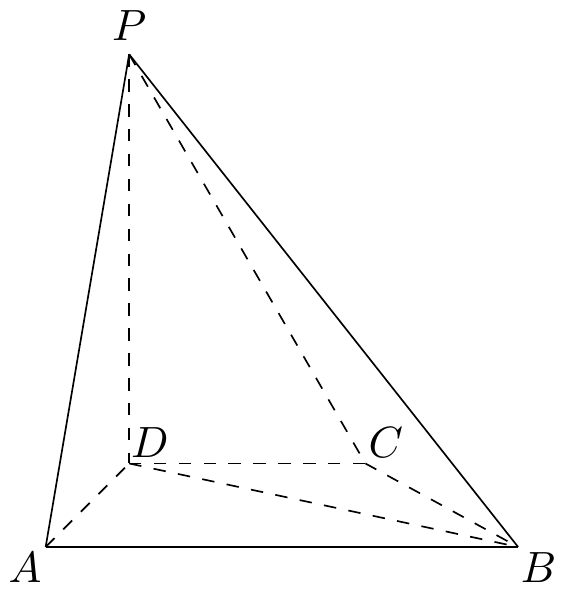
\includegraphics[width=6.6cm]{GaoKao/images/2022/national_paper_a_science/q18_fig1.png}
\par}

        \begin{enumerate}[label=(\arabic*)]
            \item 证明：$BD\perp PA$；
            \item 求 $PD$ 与平面 $PAB$ 所成的角的正弦值．
        \end{enumerate}

        \item （12分）

        甲、乙两个学校进行体育比赛，比赛共设三个项目，每个项目胜方得10分，负方得0分，没有平局．三个项目比赛结束后，总得分高的学校获得冠军．已知甲学校在三个项目中获胜的概率分别为 $0.5,0.4,0.8$，各项目的比赛结果相互独立．

        \begin{enumerate}[label=(\arabic*)]
            \item 求甲学校获得冠军的概率；
            \item 用 $X$ 表示乙学校的总得分，求 $X$ 的分布列与期望．
        \end{enumerate}

        \item （12分）

        设抛物线 $C:y^2=2px\,(p>0)$ 的焦点为 $F$，点 $D(p,0)$，过 $F$ 的直线交 $C$ 于 $M,N$ 两点．当直线 $MD$ 垂直于 $x$ 轴时，$|MF|=3$．

        \begin{enumerate}[label=(\arabic*)]
            \item 求 $C$ 的方程；
            \item 设直线 $MD,ND$ 与 $C$ 的另一个交点分别为 $A,B$，记直线 $MN,AB$ 的倾斜角分别为 $\alpha,\beta$．当 $\alpha-\beta$ 取得最大值时，求直线 $AB$ 的方程．
        \end{enumerate}

        \item （12分）

        已知函数 $f(x)=\dfrac{\mathrm{e}^x}{x}-\ln x+x-a$．

        \begin{enumerate}[label=(\arabic*)]
            \item 若 $f(x)\geqslant0$，求 $a$ 的取值范围；
            \item 证明：若 $f(x)$ 有两个零点 $x_1,x_2$，则 $x_1x_2<1$．
        \end{enumerate}

        \item （10分）[选修4-4：坐标系与参数方程]

        在直角坐标系 $xOy$ 中，曲线 $C_1$ 的参数方程为 $\begin{cases}x=\dfrac{2+t}{6},\\y=\sqrt{t}\end{cases}$（$t$ 为参数），曲线 $C_2$ 的参数方程为 $\begin{cases}x=-\dfrac{2+s}{6},\\y=-\sqrt{s}\end{cases}$（$s$ 为参数）．

        \begin{enumerate}[label=(\arabic*)]
            \item 写出 $C_1$ 的普通方程；
            \item 以坐标原点为极点，$x$ 轴正半轴为极轴建立极坐标系，曲线 $C_3$ 的极坐标方程为 $2\cos\theta-\sin\theta=0$，求 $C_3$ 与 $C_1$ 交点的直角坐标，及 $C_3$ 与 $C_2$ 交点的直角坐标．
        \end{enumerate}

        \item （10分）[选修4-5：不等式选讲]

        已知 $a,b,c$ 均为正数，且 $a^2+b^2+4c^2=3$，证明：

        \begin{enumerate}[label=(\arabic*)]
            \item $a+b+2c\leqslant3$；
            \item 若 $b=2c$，则 $\dfrac{1}{a}+\dfrac{1}{c}\geqslant3$．
        \end{enumerate}
    \end{enumerate}
\end{description}
\clearpage


\subsection{2022年全国甲卷（文）}\label{gk:2022年全国甲卷（文）}

\begin{description}
    \item[一、选择题] 本题共12小题，每小题5分，共60分．在每小题给出的四个选项中，只有一项是符合题目要求的．
    \begin{enumerate}[leftmargin=5pt]
        \item 设集合 $A=\{-2,-1,0,1,2\}$，$B=\bigl\{x\mid0\leqslant x<\frac{5}{2}\bigr\}$，则 $A\cap B=$
       
        {\centering\begin{tabular*}{\linewidth}{@{}@{\extracolsep{\fill}}llll@{}}
          \(\text{A. }\{0,1,2\}\)  & \(\text{B. }\{-2,-1,0\}\)  & \(\text{C. }\{0,1\}\)  & \(\text{D. }\{1,2\}\)
        \end{tabular*}\par}

        \item 某社区通过公益讲座以普及社区居民的垃圾分类知识．为了解讲座效果，随机抽取10位社区居民，让他们在讲座前和讲座后各回答一份垃圾分类知识问卷，这10位社区居民在讲座前和讲座后问卷答题的正确率如下图：
        
        {\centering
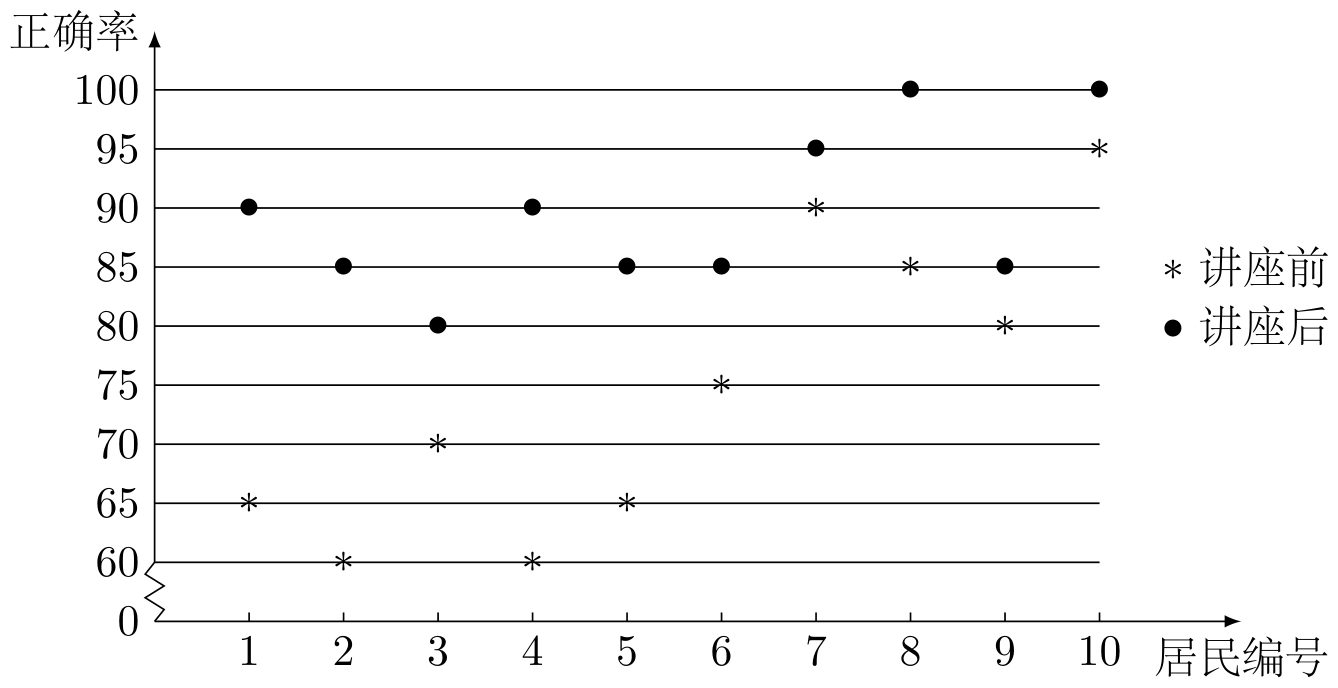
\includegraphics[width=12.8cm]{GaoKao/images/2022/national_paper_a_liberal/q2_fig1.png}
\par}

        则
       
        {\centering\begin{tabular*}{\linewidth}{@{}@{\extracolsep{\fill}}llll@{}}
          \(\text{A. }\)讲座前问卷答题的正确率的中位数小于$70\%$ \\
          \(\text{B. }\)讲座后问卷答题的正确率的平均数大于$85\%$ \\
          \(\text{C. }\)讲座前问卷答题的正确率的标准差小于讲座后正确率的标准差 \\
          \(\text{D. }\)讲座后问卷答题的正确率的极差大于讲座前正确率的极差
        \end{tabular*}\par}

        \item 若 $z=1+\i$，则 $|\i z+3\bar{z}|=$
       
        {\centering\begin{tabular*}{\linewidth}{@{}@{\extracolsep{\fill}}llll@{}}
          \(\text{A. }4\sqrt{5}\)  & \(\text{B. }4\sqrt{2}\)  & \(\text{C. }2\sqrt{5}\)  & \(\text{D. }2\sqrt{2}\)
        \end{tabular*}\par}

        \item 如图，网格纸上绘制的是一个多面体的三视图，网格小正方形的边长为1，则该多面体的体积为
        
        {\centering
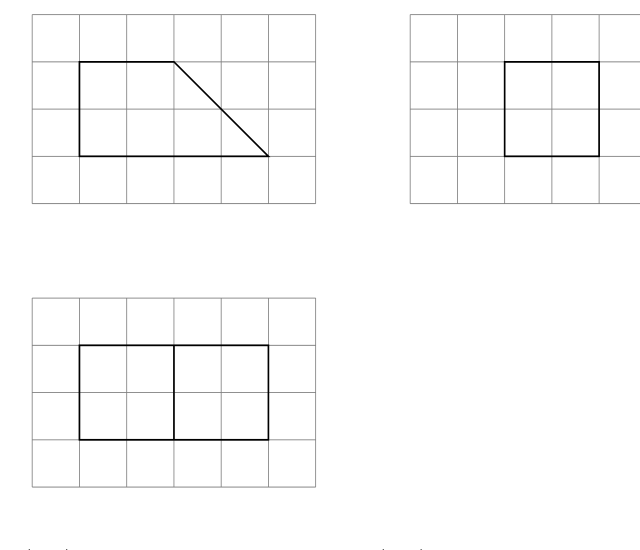
\includegraphics[width=6.0cm]{GaoKao/images/2022/national_paper_a_liberal/q4_fig1.png}
\par}

        {\centering\begin{tabular*}{\linewidth}{@{}@{\extracolsep{\fill}}llll@{}}
          \(\text{A. }8\)  & \(\text{B. }12\)  & \(\text{C. }16\)  & \(\text{D. }20\)
        \end{tabular*}\par}

        \item 将函数 $f(x)=\sin\bigl(\omega x+\frac{\pi}{3}\bigr)\,(\omega>0)$ 的图像向左平移 $\frac{\pi}{2}$ 个单位长度后得到曲线 $C$，若 $C$ 关于 $y$ 轴对称，则 $\omega$ 的最小值是
       
        {\centering\begin{tabular*}{\linewidth}{@{}@{\extracolsep{\fill}}llll@{}}
          \(\text{A. }\dfrac{1}{6}\)  & \(\text{B. }\dfrac{1}{4}\)  & \(\text{C. }\dfrac{1}{3}\)  & \(\text{D. }\dfrac{1}{2}\)
        \end{tabular*}\par}

        \item 从分别写有 $1,2,3,4,5,6$ 的6张卡片中无放回随机抽取2张，则抽到的2张卡片上的数字之积是4的倍数的概率为
       
        {\centering\begin{tabular*}{\linewidth}{@{}@{\extracolsep{\fill}}llll@{}}
          \(\text{A. }\dfrac{1}{5}\)  & \(\text{B. }\dfrac{1}{3}\)  & \(\text{C. }\dfrac{2}{5}\)  & \(\text{D. }\dfrac{2}{3}\)
        \end{tabular*}\par}

        \item 函数 $y=(3^x-3^{-x})\cos x$ 在区间 $\bigl[-\frac{\pi}{2},\frac{\pi}{2}\bigr]$ 的图象大致为
        
        {\centering
            \begin{tabular*}{\linewidth}{@{}@{\extracolsep{\fill}}cccc@{}}
            \(\text{A. }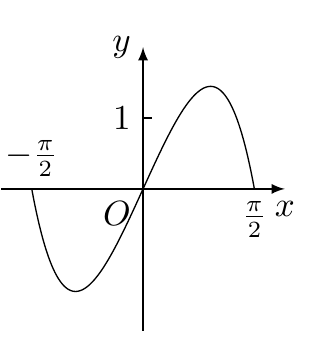
\includegraphics[width=0.15\paperwidth]{GaoKao/images/2022/national_paper_a_liberal/q7_optA.png}\)  &  \(\text{B. }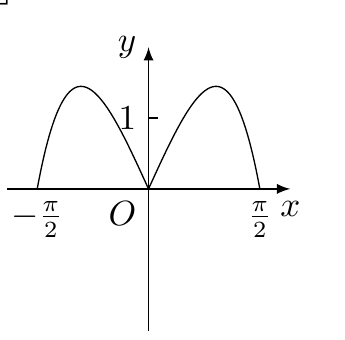
\includegraphics[width=0.15\paperwidth]{GaoKao/images/2022/national_paper_a_liberal/q7_optB.png}\)  &  \(\text{C. }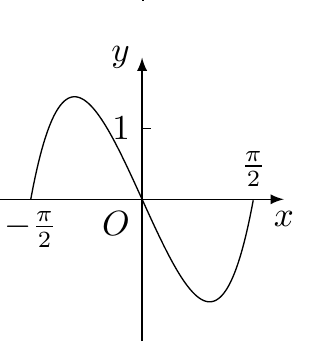
\includegraphics[width=0.15\paperwidth]{GaoKao/images/2022/national_paper_a_liberal/q7_optC.png}\)  &  \(\text{D. }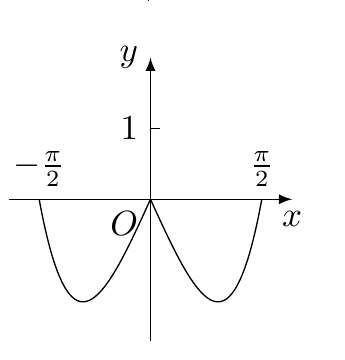
\includegraphics[width=0.15\paperwidth]{GaoKao/images/2022/national_paper_a_liberal/q7_optD.png}\)
        \end{tabular*}
        \par}

        \item 当 $x=1$ 时，函数 $f(x)=a\ln x+\dfrac{b}{x}$ 取得最大值 $-2$，则 $f'(2)=$
       
        {\centering\begin{tabular*}{\linewidth}{@{}@{\extracolsep{\fill}}llll@{}}
          \(\text{A. }-1\)  & \(\text{B. }-\dfrac{1}{2}\)  & \(\text{C. }\dfrac{1}{2}\)  & \(\text{D. }1\)
        \end{tabular*}\par}

        \item 在长方体 $ABCD$-$A_1B_1C_1D_1$ 中，已知 $B_1D$ 与平面 $ABCD$ 和平面 $AA_1B_1B$ 所成的角均为 $30^\circ$，则
       
        {\centering\begin{tabular*}{\linewidth}{@{}@{\extracolsep{\fill}}llll@{}}
          \(\text{A. }AB=2AD\)  & \(\text{B. }AB$ 与平面 $AB_1C_1D$ 所成的角为 $30^\circ$ \\
          \(\text{C. }AC=CB_1\)  & \(\text{D. }B_1D$ 与平面 $BB_1C_1C$ 所成的角为 $45^\circ\)
        \end{tabular*}\par}

        \item 甲、乙两个圆锥的母线长相等，侧面展开图的圆心角之和为 $2\pi$，侧面积分别为 $S_{\text{甲}}$ 和 $S_{\text{乙}}$，体积分别为 $V_{\text{甲}}$ 和 $V_{\text{乙}}$．若 $\dfrac{S_{\text{甲}}}{S_{\text{乙}}}=2$，则 $\dfrac{V_{\text{甲}}}{V_{\text{乙}}}=$
       
        {\centering\begin{tabular*}{\linewidth}{@{}@{\extracolsep{\fill}}llll@{}}
          \(\text{A. }\sqrt{5}\)  & \(\text{B. }2\sqrt{2}\)  & \(\text{C. }\sqrt{10}\)  & \(\text{D. }\dfrac{5\sqrt{10}}{4}\)
        \end{tabular*}\par}

        \item 已知椭圆 $C:\dfrac{x^2}{a^2}+\dfrac{y^2}{b^2}=1\,(a>b>0)$ 的离心率为 $\dfrac{1}{3}$，$A_1,A_2$ 分别为 $C$ 的左、右顶点，$B$ 为 $C$ 的上顶点．若 $\overrightarrow{BA_1}\cdot\overrightarrow{BA_2}=-1$，则 $C$ 的方程为
       
        {\centering\begin{tabular*}{\linewidth}{@{}@{\extracolsep{\fill}}llll@{}}
          \(\text{A. }\dfrac{x^2}{18}+\dfrac{y^2}{16}=1\)  & \(\text{B. }\dfrac{x^2}{9}+\dfrac{y^2}{8}=1\)  & \(\text{C. }\dfrac{x^2}{3}+\dfrac{y^2}{2}=1\)  & \(\text{D. }\dfrac{x^2}{18}+y^2=1\)
        \end{tabular*}\par}

        \item 已知 $9^m=10$，$a=10^m-11$，$b=8^m-9$，则
       
        {\centering\begin{tabular*}{\linewidth}{@{}@{\extracolsep{\fill}}llll@{}}
          \(\text{A. }a>0>b\)  & \(\text{B. }a>b>0\)  & \(\text{C. }b>a>0\)  & \(\text{D. }b>0>a\)
        \end{tabular*}\par}
    \end{enumerate}
\end{description}

\begin{description}
    \item[二、填空题] 本题共4小题，每小题5分，共20分．
    \begin{enumerate}[leftmargin=5pt]
      \addtocounter{enumi}{+12}
        \item 记 $S_n$ 为等差数列 $\{a_n\}$ 的前 $n$ 项和．若 $2S_3=3S_2+6$，则公差 $d=$ \rule[-0.3ex]{3em}{0.4pt}．
        \item 从甲、乙等5名同学中随机选3名参加社区服务工作，则甲、乙都入选的概率为 \rule[-0.3ex]{3em}{0.4pt}．
        \item 过四点 $(0,0),(4,0),(-1,1),(4,2)$ 中的三点的一个圆的方程为 \rule[-0.3ex]{3em}{0.4pt}．
        \item 若 $x=\ln\dfrac{1}{2}$ 是函数 $f(x)=a\mathrm{e}^{2x}+\dfrac{x-1}{x}$ 的极值点，则 $a$ 的值为 \rule[-0.3ex]{3em}{0.4pt}．$f(x)$ 的零点个数为 \rule[-0.3ex]{3em}{0.4pt}．
    \end{enumerate}
\end{description}

\begin{description}
    \item[三、解答题] 本题共7小题，共70分．解答应写出文字说明、证明过程或演算步骤．第17\textasciitilde21题为必考题，第22、23题为选考题．
    \begin{enumerate}[leftmargin=5pt]
      \addtocounter{enumi}{+16}
        \item （12分）

        甲、乙两城之间的长途客车均由 $A$ 和 $B$ 两家公司运营．为了解这两家公司长途客车的运行情况，随机调查了甲、乙两城之间的500个班次，得到下面列联表：

        {\centering\begin{tabular}{c|c|c}
        \hline
        & 准点班次数 & 未准点班次数 \\
        \hline
        $A$ & 240 & 20 \\
        \hline
        $B$ & 210 & 30 \\
        \hline
        \end{tabular}\par}

        \begin{enumerate}[label=(\arabic*)]
            \item 根据上表，分别估计这两家公司甲、乙两城之间的长途客车准点的概率；
            \item 能否有 $90\%$ 的把握认为甲、乙两城之间的长途客车是否准点与客车所属公司有关？

            附：$K^2=\dfrac{n(ad-bc)^2}{(a+b)(c+d)(a+c)(b+d)}$，$P(K^2\geqslant k)$：0.100--2.706，0.050--3.841．
        \end{enumerate}

        \item （12分）

        记 $S_n$ 为数列 $\{a_n\}$ 的前 $n$ 项和．已知 $\dfrac{2S_n}{n}+n=2a_n+1$．

        \begin{enumerate}[label=(\arabic*)]
            \item 证明：$\{a_n\}$ 是等差数列；
            \item 若 $a_4,a_7,a_9$ 成等比数列，求 $S_n$ 的最小值．
        \end{enumerate}

        \item （12分）

        小明同学参加综合实践活动，设计了一个封闭的包装盒．包装盒如图所示：底面 $ABCD$ 是边长为8（单位：cm）的正方形，$\triangle EAB,\triangle FBC,\triangle GCD,\triangle HDA$ 均为正三角形，且它们所在的平面都与平面 $ABCD$ 垂直．

        {\centering
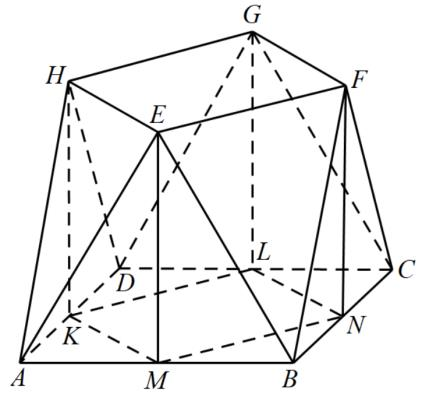
\includegraphics[width=10.7cm]{GaoKao/images/2022/national_paper_a_liberal/q19_fig1.png}
\par}

        \begin{enumerate}[label=(\arabic*)]
            \item 证明：$EF\parallel$ 平面 $ABCD$；
            \item 求该包装盒的容积（忽略包装盒材料的厚度）．
        \end{enumerate}

        \item （12分）

        已知函数 $f(x)=x^3-x$，$g(x)=x^2+a$，曲线 $y=f(x)$ 在点 $(x_1,f(x_1))$ 处的切线也是曲线 $y=g(x)$ 的切线．

        \begin{enumerate}[label=(\arabic*)]
            \item 若 $x_1=-1$，求 $a$；
            \item 求 $a$ 的取值范围．
        \end{enumerate}

        \item （12分）

        设抛物线 $C:y^2=2px\,(p>0)$ 的焦点为 $F$，点 $D(p,0)$，过 $F$ 的直线交 $C$ 于 $M,N$ 两点．当直线 $MD$ 垂直于 $x$ 轴时，$|MF|=3$．

        \begin{enumerate}[label=(\arabic*)]
            \item 求 $C$ 的方程；
            \item 设直线 $MD,ND$ 与 $C$ 的另一个交点分别为 $A,B$，记直线 $MN,AB$ 的倾斜角分别为 $\alpha,\beta$．当 $\alpha-\beta$ 取得最大值时，求直线 $AB$ 的方程．
        \end{enumerate}

        \item （10分）[选修4-4：坐标系与参数方程]

        在直角坐标系 $xOy$ 中，曲线 $C_1$ 的参数方程为 $\begin{cases}x=\dfrac{2+t}{6},\\y=\sqrt{t}\end{cases}$（$t$ 为参数），曲线 $C_2$ 的参数方程为 $\begin{cases}x=-\dfrac{2+s}{6},\\y=-\sqrt{s}\end{cases}$（$s$ 为参数）．

        \begin{enumerate}[label=(\arabic*)]
            \item 写出 $C_1$ 的普通方程；
            \item 以坐标原点为极点，$x$ 轴正半轴为极轴建立极坐标系，曲线 $C_3$ 的极坐标方程为 $2\cos\theta-\sin\theta=0$，求 $C_3$ 与 $C_1$ 交点的直角坐标，及 $C_3$ 与 $C_2$ 交点的直角坐标．
        \end{enumerate}

        \item （10分）[选修4-5：不等式选讲]

        已知 $a,b,c$ 均为正数，且 $a^2+b^2+4c^2=3$，证明：

        \begin{enumerate}[label=(\arabic*)]
            \item $a+b+2c\leqslant3$；
            \item 若 $b=2c$，则 $\dfrac{1}{a}+\dfrac{1}{c}\geqslant3$．
        \end{enumerate}
    \end{enumerate}
\end{description}
\clearpage


\subsection{2022年全国乙卷（理）}\label{gk:2022年全国乙卷（理）}

\begin{description}
    \item[一、选择题] 本题共12小题，每小题5分，共60分．在每小题给出的四个选项中，只有一项是符合题目要求的．
    \begin{enumerate}[leftmargin=5pt]
        \item 设全集 $U=\{1,2,3,4,5\}$，集合 $M$ 满足 $\complement_U M=\{1,3\}$，则
       
        {\centering\begin{tabular*}{\linewidth}{@{}@{\extracolsep{\fill}}llll@{}}
          \(\text{A. }2\in M\)  & \(\text{B. }3\in M\)  & \(\text{C. }4\notin M\)  & \(\text{D. }5\notin M\)
        \end{tabular*}\par}

        \item 已知 $z=1-2\i$，且 $z+a\bar{z}+b=0$，其中 $a,b$ 为实数，则
       
        {\centering\begin{tabular*}{\linewidth}{@{}@{\extracolsep{\fill}}llll@{}}
          \(\text{A. }a=1,b=-2\)  & \(\text{B. }a=-1,b=2\)  & \(\text{C. }a=1,b=2\)  & \(\text{D. }a=-1,b=-2\)
        \end{tabular*}\par}

        \item 已知向量 $\bm a,\bm b$ 满足 $|\bm a|=1$，$|\bm b|=\sqrt{3}$，$|\bm a-2\bm b|=3$，则 $\bm a\cdot\bm b=$
       
        {\centering\begin{tabular*}{\linewidth}{@{}@{\extracolsep{\fill}}llll@{}}
          \(\text{A. }-2\)  & \(\text{B. }-1\)  & \(\text{C. }1\)  & \(\text{D. }2\)
        \end{tabular*}\par}

        \item 嫦娥二号卫星在完成探月任务后，继续进行深空探测，成为我国第一颗环绕太阳飞行的人造行星．为研究嫦娥二号绕日周期与地球绕日周期的比值，用到数列 $\{b_n\}$：$b_1=1+\dfrac{1}{\alpha_1}$，$b_2=1+\dfrac{1}{\alpha_1+\dfrac{1}{\alpha_2}}$，$b_3=1+\dfrac{1}{\alpha_1+\dfrac{1}{\alpha_2+\dfrac{1}{\alpha_3}}}$，$\cdots$，依此类推，其中 $\alpha_k\in\mathbb{N}^*\,(k=1,2,\cdots)$．则
       
        {\centering\begin{tabular*}{\linewidth}{@{}@{\extracolsep{\fill}}llll@{}}
          \(\text{A. }b_1<b_3<b_5\)  & \(\text{B. }b_3<b_8<b_5\)  & \(\text{C. }b_6<b_2<b_8\)  & \(\text{D. }b_4<b_7<b_2\)
        \end{tabular*}\par}

        \item 设 $F$ 为抛物线 $C:y^2=4x$ 的焦点，点 $A$ 在 $C$ 上，点 $B(3,0)$，若 $|AF|=|BF|$，则 $|AB|=$
       
        {\centering\begin{tabular*}{\linewidth}{@{}@{\extracolsep{\fill}}llll@{}}
          \(\text{A. }2\)  & \(\text{B. }2\sqrt{2}\)  & \(\text{C. }3\)  & \(\text{D. }3\sqrt{2}\)
        \end{tabular*}\par}

        \item 执行下面的程序框图，输出的 $n=$
        
        {\centering
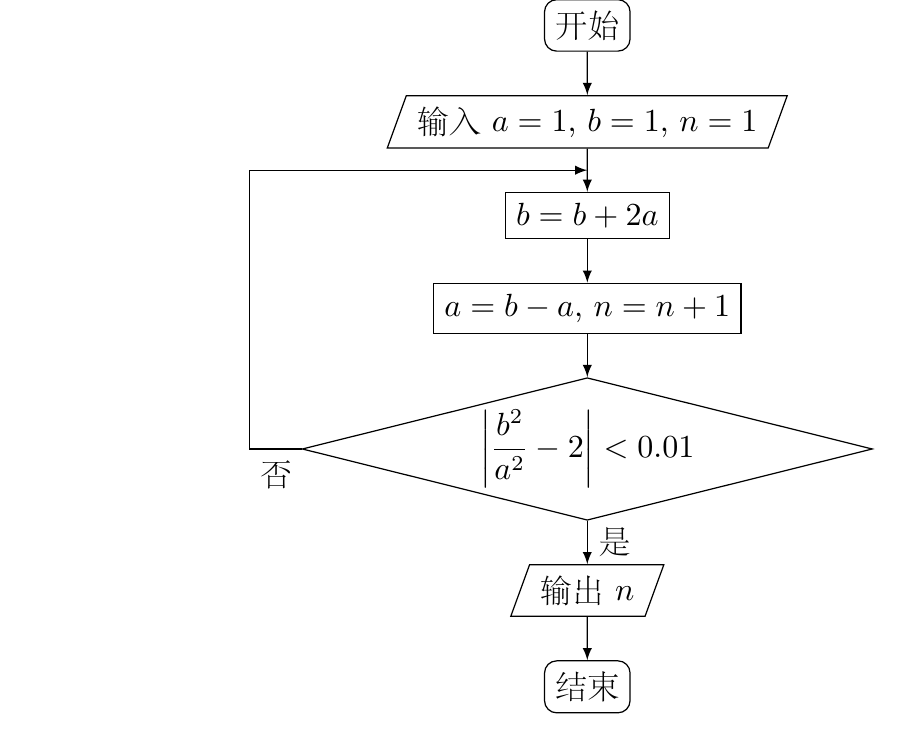
\includegraphics[width=0.65\linewidth]{GaoKao/images/2022/national_paper_b_science/q6_fig1.png}
\par}

        {\centering\begin{tabular*}{\linewidth}{@{}@{\extracolsep{\fill}}llll@{}}
          \(\text{A. }3\)  & \(\text{B. }4\)  & \(\text{C. }5\)  & \(\text{D. }6\)
        \end{tabular*}\par}

        \item 在正方体 $ABCD$-$A_1B_1C_1D_1$ 中，$E,F$ 分别为 $AB,BC$ 的中点，则
       
        {\centering\begin{tabular*}{\linewidth}{@{}@{\extracolsep{\fill}}llll@{}}
          \(\text{A. }\)平面 $B_1EF\perp$ 平面 $BDD_1$  & \(\text{B. }\)平面 $B_1EF\perp$ 平面 $A_1BD$ \\
          \(\text{C. }\)平面 $B_1EF\parallel$ 平面 $A_1AC$  & \(\text{D. }\)平面 $B_1EF\parallel$ 平面 $A_1C_1D$
        \end{tabular*}\par}

        \item 已知等比数列 $\{a_n\}$ 的前3项和为168，$a_2-a_5=42$，则 $a_6=$
       
        {\centering\begin{tabular*}{\linewidth}{@{}@{\extracolsep{\fill}}llll@{}}
          \(\text{A. }14\)  & \(\text{B. }12\)  & \(\text{C. }6\)  & \(\text{D. }3\)
        \end{tabular*}\par}

        \item 已知球 $O$ 的半径为1，四棱锥的顶点为 $O$，底面的四个顶点均在球 $O$ 的球面上，则当该四棱锥的体积最大时，其高为
       
        {\centering\begin{tabular*}{\linewidth}{@{}@{\extracolsep{\fill}}llll@{}}
          \(\text{A. }\dfrac{1}{3}\)  & \(\text{B. }\dfrac{1}{2}\)  & \(\text{C. }\dfrac{\sqrt{3}}{3}\)  & \(\text{D. }\dfrac{\sqrt{2}}{2}\)
        \end{tabular*}\par}

        \item 某棋手与甲、乙、丙三位棋手各比赛一盘，各盘比赛结果相互独立．已知该棋手与甲、乙、丙比赛获胜的概率分别为 $p_1,p_2,p_3$，且 $p_3>p_2>p_1>0$．记该棋手连胜两盘的概率为 $p$，则
       
        {\centering\begin{tabular*}{\linewidth}{@{}@{\extracolsep{\fill}}llll@{}}
          \(\text{A. }p$ 与该棋手和甲、乙、丙的比赛次序无关  & \(\text{B. }\)该棋手在第二盘与甲比赛，$p$ 最大 \\
          \(\text{C. }\)该棋手在第二盘与乙比赛，$p$ 最大  & \(\text{D. }\)该棋手在第二盘与丙比赛，$p$ 最大
        \end{tabular*}\par}

        \item 双曲线 $C$ 的两个焦点为 $F_1,F_2$，以 $C$ 的实轴为直径的圆记为 $D$，过 $F_1$ 作 $D$ 的切线与 $C$ 的两支分别交于 $M,N$ 两点，且 $\cos\angle F_1NF_2=\dfrac{3}{5}$，则 $C$ 的离心率为
       
        {\centering\begin{tabular*}{\linewidth}{@{}@{\extracolsep{\fill}}llll@{}}
          \(\text{A. }\dfrac{\sqrt{5}}{2}\)  & \(\text{B. }\dfrac{3}{2}\)  & \(\text{C. }\dfrac{\sqrt{13}}{2}\)  & \(\text{D. }\dfrac{\sqrt{17}}{2}\)
        \end{tabular*}\par}

        \item 已知函数 $f(x),g(x)$ 的定义域均为 $\mathbb{R}$，且 $f(x)+g(2-x)=5$，$g(x)-f(x-4)=7$．若 $y=g(x)$ 的图像关于直线 $x=2$ 对称，$g(2)=4$，则 $\displaystyle\sum_{k=1}^{22}f(k)=$
       
        {\centering\begin{tabular*}{\linewidth}{@{}@{\extracolsep{\fill}}llll@{}}
          \(\text{A. }-21\)  & \(\text{B. }-22\)  & \(\text{C. }-23\)  & \(\text{D. }-24\)
        \end{tabular*}\par}
    \end{enumerate}
\end{description}

\begin{description}
    \item[二、填空题] 本题共4小题，每小题5分，共20分．
    \begin{enumerate}[leftmargin=5pt]
      \addtocounter{enumi}{+12}
        \item 从甲、乙等5名同学中随机选3名参加社区服务工作，则甲、乙都入选的概率为 \rule[-0.3ex]{3em}{0.4pt}．
        \item 过四点 $(0,0),(4,0),(-1,1),(4,2)$ 中的三点的一个圆的方程为 \rule[-0.3ex]{3em}{0.4pt}．
        \item 记函数 $f(x)=\cos(\omega x+\varphi)\,(\omega>0,0<\varphi<\pi)$ 的最小正周期为 $T$．若 $f(T)=\dfrac{\sqrt{3}}{2}$，$x=\dfrac{\pi}{9}$ 为 $f(x)$ 的零点，则 $\omega$ 的最小值为 \rule[-0.3ex]{3em}{0.4pt}．
        \item 已知 $x=x_1$ 和 $x=x_2$ 分别是函数 $f(x)=2a^x-\mathrm{e} x^2\,(a>0$ 且 $a\neq1)$ 的极小值点和极大值点．若 $x_1<x_2$，则 $a$ 的取值范围是 \rule[-0.3ex]{3em}{0.4pt}．
    \end{enumerate}
\end{description}

\begin{description}
    \item[三、解答题] 本题共7小题，共70分．解答应写出文字说明、证明过程或演算步骤．第17\textasciitilde21题为必考题，第22、23题为选考题．
    \begin{enumerate}[leftmargin=5pt]
      \addtocounter{enumi}{+16}
        \item （12分）

        记 $\triangle ABC$ 的内角 $A,B,C$ 的对边分别为 $a,b,c$，已知 $\sin C\sin(A-B)=\sin B\sin(C-A)$．

        \begin{enumerate}[label=(\arabic*)]
            \item 证明：$2a^2=b^2+c^2$；
            \item 若 $a=5$，$\cos A=\dfrac{25}{31}$，求 $\triangle ABC$ 的周长．
        \end{enumerate}

        \item （12分）

        如图，四面体 $ABCD$ 中，$AD\perp CD$，$AD=CD$，$\angle ADB=\angle BDC$，$E$ 为 $AC$ 的中点．

        {\centering
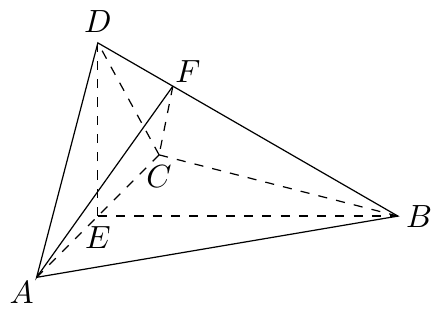
\includegraphics[width=7.3cm]{GaoKao/images/2022/national_paper_b_science/q18_fig1.png}
\par}

        \begin{enumerate}[label=(\arabic*)]
            \item 证明：平面 $BED\perp$ 平面 $ACD$；
            \item 设 $AB=BD=2$，$\angle ACB=60^\circ$，点 $F$ 在 $BD$ 上，当 $\triangle AFC$ 的面积最小时，求 $CF$ 与平面 $ABD$ 所成的角的正弦值．
        \end{enumerate}

        \item （12分）

        某地经过多年的环境治理，已将荒山改造成了绿水青山．为估计一林区某种树木的总材积量，随机选取了10棵这种树木，测量每棵树的根部横截面积（单位：$\text{m}^2$）和材积量（单位：$\text{m}^3$），得到如下数据：

        \textsf{[插入表格：10棵树数据]}

        并计算得 $\sum x_i^2=0.038$，$\sum y_i^2=1.6158$，$\sum x_iy_i=0.2474$．

        \begin{enumerate}[label=(\arabic*)]
            \item 估计该林区这种树木平均一棵的根部横截面积与平均一棵的材积量；
            \item 求该林区这种树木的根部横截面积与材积量的样本相关系数（精确到0.01）；
            \item 现测量了该林区所有这种树木的根部横截面积，并得到所有这种树木的根部横截面积总和为 $186\,\text{m}^2$．已知树木的材积量与其根部横截面积近似成正比．利用以上数据给出该林区这种树木的总材积量的估计值．

            附：相关系数 $r=\dfrac{\sum(x_i-\bar{x})(y_i-\bar{y})}{\sqrt{\sum(x_i-\bar{x})^2\sum(y_i-\bar{y})^2}}$，$\sqrt{1.896}\approx1.377$．
        \end{enumerate}

        \item （12分）

        已知椭圆 $E$ 的中心为坐标原点，对称轴为 $x$ 轴、$y$ 轴，且过 $A(0,-2)$，$B\bigl(\frac{3}{2},-1\bigr)$ 两点．

        \begin{enumerate}[label=(\arabic*)]
            \item 求 $E$ 的方程；
            \item 设过点 $P(1,-2)$ 的直线交 $E$ 于 $M,N$ 两点，过 $M$ 且平行于 $x$ 轴的直线与线段 $AB$ 交于点 $T$，点 $H$ 满足 $\overrightarrow{MT}=\overrightarrow{TH}$．证明：直线 $HN$ 过定点．
        \end{enumerate}

        \item （12分）

        已知函数 $f(x)=\ln(1+x)+ax\mathrm{e}^{-x}$．

        \begin{enumerate}[label=(\arabic*)]
            \item 当 $a=1$ 时，求曲线 $y=f(x)$ 在点 $(0,f(0))$ 处的切线方程；
            \item 若 $f(x)$ 在区间 $(-1,0),(0,+\infty)$ 各恰有一个零点，求 $a$ 的取值范围．
        \end{enumerate}

        \item （10分）[选修4-4：坐标系与参数方程]

        在直角坐标系 $xOy$ 中，曲线 $C$ 的参数方程为 $\begin{cases}x=\sqrt{3}\cos2t,\\y=2\sin t\end{cases}$（$t$ 为参数）．以坐标原点为极点，$x$ 轴正半轴为极轴建立极坐标系，已知直线 $l$ 的极坐标方程为 $\rho\sin\bigl(\theta+\frac{\pi}{3}\bigr)+m=0$．

        \begin{enumerate}[label=(\arabic*)]
            \item 写出 $l$ 的直角坐标方程；
            \item 若 $l$ 与 $C$ 有公共点，求 $m$ 的取值范围．
        \end{enumerate}

        \item （10分）[选修4-5：不等式选讲]

        已知 $a,b,c$ 都是正数，且 $a^{\frac{3}{2}}+b^{\frac{3}{2}}+c^{\frac{3}{2}}=1$，证明：

        \begin{enumerate}[label=(\arabic*)]
            \item $abc\leqslant\dfrac{1}{9}$；
            \item $\dfrac{a}{b+c}+\dfrac{b}{a+c}+\dfrac{c}{a+b}\leqslant\dfrac{1}{2\sqrt{abc}}$．
        \end{enumerate}
    \end{enumerate}
\end{description}
\clearpage


\subsection{2022年全国乙卷（文）}\label{gk:2022年全国乙卷（文）}

\begin{description}
    \item[一、选择题] 本题共12小题，每小题5分，共60分．在每小题给出的四个选项中，只有一项是符合题目要求的．
    \begin{enumerate}[leftmargin=5pt]
        \item 集合 $M=\{2,4,6,8,10\}$，$N=\{x\mid -1<x<6\}$，则 $M\cap N=$
       
        {\centering\begin{tabular*}{\linewidth}{@{}@{\extracolsep{\fill}}llll@{}}
          \(\text{A. }\{2,4\}\)  & \(\text{B. }\{2,4,6\}\)  & \(\text{C. }\{2,4,6,8\}\)  & \(\text{D. }\{2,4,6,8,10\}\)
        \end{tabular*}\par}

        \item 设 $(1+2\i)a+b=2\i$，其中 $a,b$ 为实数，则
       
        {\centering\begin{tabular*}{\linewidth}{@{}@{\extracolsep{\fill}}llll@{}}
          \(\text{A. }a=1,b=-1\)  & \(\text{B. }a=1,b=1\)  & \(\text{C. }a=-1,b=1\)  & \(\text{D. }a=-1,b=-1\)
        \end{tabular*}\par}

        \item 已知向量 $\bm a=(2,1)$，$\bm b=(-2,4)$，则 $|\bm a-\bm b|=$
       
        {\centering\begin{tabular*}{\linewidth}{@{}@{\extracolsep{\fill}}llll@{}}
          \(\text{A. }2\)  & \(\text{B. }3\)  & \(\text{C. }4\)  & \(\text{D. }5\)
        \end{tabular*}\par}

        \item 分别统计了甲、乙两位同学16周的各周课外体育运动时长（单位：h），得如下茎叶图：
        
        \begin{center}
\begin{tabular}{r|c|l}
甲 & 茎 & 乙 \\
\hline
$6\quad1$ & $5.$ & \\
$8\quad5\quad3\quad0$ & $6.$ & $3$ \\
$7\quad5\quad3\quad2$ & $7.$ & $4\quad6$ \\
$6\quad4\quad2\quad1$ & $8.$ & $1\quad2\quad2\quad5\quad6\quad6\quad6\quad6$ \\
$4\quad2$ & $9.$ & $0\quad2\quad3\quad8$ \\
 & $10.$ & $1$
\end{tabular}
\end{center}

        则下列结论中错误的是
       
        {\centering\begin{tabular*}{\linewidth}{@{}@{\extracolsep{\fill}}llll@{}}
          \(\text{A. }\)甲同学周课外体育运动时长的样本中位数为$7.4$ \\
          \(\text{B. }\)乙同学周课外体育运动时长的样本平均数大于$8$ \\
          \(\text{C. }\)甲同学周课外体育运动时长大于$8$的概率的估计值大于$0.4$ \\
          \(\text{D. }\)乙同学周课外体育运动时长大于$8$的概率的估计值大于$0.6$
        \end{tabular*}\par}

        \item 若 $x,y$ 满足约束条件 $\begin{cases}x+y\geqslant2,\\x+2y\leqslant4,\\y\geqslant0,\end{cases}$ 则 $z=2x-y$ 的最大值是
       
        {\centering\begin{tabular*}{\linewidth}{@{}@{\extracolsep{\fill}}llll@{}}
          \(\text{A. }-2\)  & \(\text{B. }4\)  & \(\text{C. }8\)  & \(\text{D. }12\)
        \end{tabular*}\par}

        \item 设 $F$ 为抛物线 $C:y^2=4x$ 的焦点，点 $A$ 在 $C$ 上，点 $B(3,0)$，若 $|AF|=|BF|$，则 $|AB|=$
       
        {\centering\begin{tabular*}{\linewidth}{@{}@{\extracolsep{\fill}}llll@{}}
          \(\text{A. }2\)  & \(\text{B. }2\sqrt{2}\)  & \(\text{C. }3\)  & \(\text{D. }3\sqrt{2}\)
        \end{tabular*}\par}

        \item 执行下面的程序框图，输出的 $n=$
        
        {\centering

\includegraphics[width=0.65\linewidth]{GaoKao/images/2022/national_paper_b_liberal/q7_fig1.png}
\par}

        {\centering\begin{tabular*}{\linewidth}{@{}@{\extracolsep{\fill}}llll@{}}
          \(\text{A. }3\)  & \(\text{B. }4\)  & \(\text{C. }5\)  & \(\text{D. }6\)
        \end{tabular*}\par}

        \item 函数 $f(x)=\dfrac{x+1}{x^2+1}$ 在区间 $[0,2]$ 上的最大值、最小值分别为
       
        {\centering\begin{tabular*}{\linewidth}{@{}@{\extracolsep{\fill}}llll@{}}
          \(\text{A. }\dfrac{3}{5},\dfrac{1}{5}\)  & \(\text{B. }\dfrac{1}{2},\dfrac{1}{5}\)  & \(\text{C. }\dfrac{1}{2},0\)  & \(\text{D. }\dfrac{3}{5},0\)
        \end{tabular*}\par}

        \item 在正方体 $ABCD$-$A_1B_1C_1D_1$ 中，$E,F$ 分别为 $AB,BC$ 的中点，则
       
        {\centering\begin{tabular*}{\linewidth}{@{}@{\extracolsep{\fill}}llll@{}}
          \(\text{A. }\)平面 $B_1EF\perp$ 平面 $BDD_1$  & \(\text{B. }\)平面 $B_1EF\perp$ 平面 $A_1BD$ \\
          \(\text{C. }\)平面 $B_1EF\parallel$ 平面 $A_1AC$  & \(\text{D. }\)平面 $B_1EF\parallel$ 平面 $A_1C_1D$
        \end{tabular*}\par}

        \item 已知等比数列 $\{a_n\}$ 的前3项和为168，$a_2-a_5=42$，则 $a_6=$
       
        {\centering\begin{tabular*}{\linewidth}{@{}@{\extracolsep{\fill}}llll@{}}
          \(\text{A. }14\)  & \(\text{B. }12\)  & \(\text{C. }6\)  & \(\text{D. }3\)
        \end{tabular*}\par}

        \item 函数 $f(x)=\cos x+(x+1)\sin x+1$ 在区间 $[0,2\pi]$ 的最小值、最大值分别为
       
        {\centering\begin{tabular*}{\linewidth}{@{}@{\extracolsep{\fill}}llll@{}}
          \(\text{A. }-\dfrac{\pi}{2},\dfrac{\pi}{2}\)  & \(\text{B. }-\dfrac{3\pi}{2},\dfrac{\pi}{2}\)  & \(\text{C. }-\dfrac{\pi}{2},\dfrac{\pi}{2}+2\)  & \(\text{D. }-\dfrac{3\pi}{2},\dfrac{\pi}{2}+2\)
        \end{tabular*}\par}

        \item 已知球 $O$ 的半径为1，四棱锥的顶点为 $O$，底面的四个顶点均在球 $O$ 的球面上，则当该四棱锥的体积最大时，其高为
       
        {\centering\begin{tabular*}{\linewidth}{@{}@{\extracolsep{\fill}}llll@{}}
          \(\text{A. }\dfrac{1}{3}\)  & \(\text{B. }\dfrac{1}{2}\)  & \(\text{C. }\dfrac{\sqrt{3}}{3}\)  & \(\text{D. }\dfrac{\sqrt{2}}{2}\)
        \end{tabular*}\par}
    \end{enumerate}
\end{description}

\begin{description}
    \item[二、填空题] 本题共4小题，每小题5分，共20分．
    \begin{enumerate}[leftmargin=5pt]
      \addtocounter{enumi}{+12}
        \item 记 $S_n$ 为等差数列 $\{a_n\}$ 的前 $n$ 项和．若 $2S_3=3S_2+6$，则公差 $d=$ \rule[-0.3ex]{3em}{0.4pt}．
        \item 从甲、乙等5名同学中随机选3名参加社区服务工作，则甲、乙都入选的概率为 \rule[-0.3ex]{3em}{0.4pt}．
        \item 过四点 $(0,0),(4,0),(-1,1),(4,2)$ 中的三点的一个圆的方程为 \rule[-0.3ex]{3em}{0.4pt}．
        \item 若 $x=\ln\dfrac{1}{2}$ 是函数 $f(x)=a\mathrm{e}^{2x}+\dfrac{x-1}{x}$ 的极值点，则 $a$ 的值为 \rule[-0.3ex]{3em}{0.4pt}．
    \end{enumerate}
\end{description}

\begin{description}
    \item[三、解答题] 本题共7小题，共70分．解答应写出文字说明、证明过程或演算步骤．第17\textasciitilde21题为必考题，第22、23题为选考题．
    \begin{enumerate}[leftmargin=5pt]
      \addtocounter{enumi}{+16}
        \item （12分）

        记 $\triangle ABC$ 的内角 $A,B,C$ 的对边分别为 $a,b,c$，已知 $\sin C\sin(A-B)=\sin B\sin(C-A)$．

        \begin{enumerate}[label=(\arabic*)]
            \item 若 $A=2B$，求 $C$；
            \item 证明：$2a^2=b^2+c^2$．
        \end{enumerate}

        \item （12分）

        如图，四面体 $ABCD$ 中，$AD\perp CD$，$AD=CD$，$\angle ADB=\angle BDC$，$E$ 为 $AC$ 的中点．

        {\centering
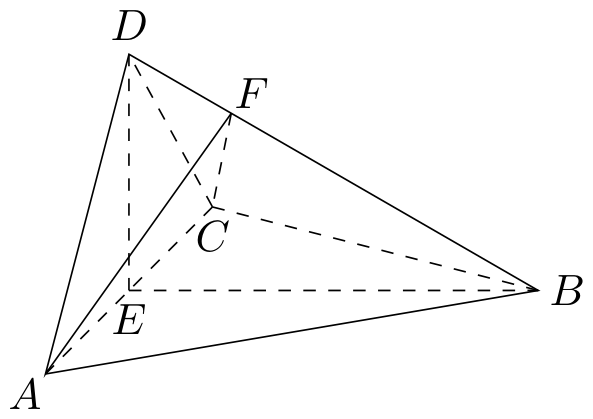
\includegraphics[width=7.2cm]{GaoKao/images/2022/national_paper_B_liberal/q18_fig1.png}
\par}

        \begin{enumerate}[label=(\arabic*)]
            \item 证明：平面 $BED\perp$ 平面 $ACD$；
            \item 设 $AB=BD=2$，$\angle ACB=60^\circ$，点 $F$ 在 $BD$ 上，当 $\triangle AFC$ 的面积最小时，求三棱锥 $F$-$ABC$ 的体积．
        \end{enumerate}

        \item （12分）

        某地经过多年的环境治理，已将荒山改造成了绿水青山．为估计一林区某种树木的总材积量，随机选取了10棵这种树木，测量每棵树的根部横截面积和材积量，得到如下数据：

        \textsf{[插入表格：10棵树数据]}

        \begin{enumerate}[label=(\arabic*)]
            \item 估计该林区这种树木平均一棵的根部横截面积与平均一棵的材积量；
            \item 求该林区这种树木的根部横截面积与材积量的样本相关系数（精确到0.01）；
            \item 现测量了该林区所有这种树木的根部横截面积，并得到所有这种树木的根部横截面积总和为 $186\,\text{m}^2$．已知树木的材积量与其根部横截面积近似成正比．利用以上数据给出该林区这种树木的总材积量的估计值．
        \end{enumerate}

        \item （12分）

        已知函数 $f(x)=ax-\dfrac{1}{x}-(a+1)\ln x$．

        \begin{enumerate}[label=(\arabic*)]
            \item 当 $a=0$ 时，求 $f(x)$ 的最大值；
            \item 若 $f(x)$ 恰有一个零点，求 $a$ 的取值范围．
        \end{enumerate}

        \item （12分）

        已知椭圆 $E$ 的中心为坐标原点，对称轴为 $x$ 轴、$y$ 轴，且过 $A(0,-2)$，$B\bigl(\frac{3}{2},-1\bigr)$ 两点．

        \begin{enumerate}[label=(\arabic*)]
            \item 求 $E$ 的方程；
            \item 设过点 $P(1,-2)$ 的直线交 $E$ 于 $M,N$ 两点，过 $M$ 且平行于 $x$ 轴的直线与线段 $AB$ 交于点 $T$，点 $H$ 满足 $\overrightarrow{MT}=\overrightarrow{TH}$．证明：直线 $HN$ 过定点．
        \end{enumerate}

        \item （10分）[选修4-4：坐标系与参数方程]

        在直角坐标系 $xOy$ 中，曲线 $C$ 的参数方程为 $\begin{cases}x=\sqrt{3}\cos2t,\\y=2\sin t\end{cases}$（$t$ 为参数）．以坐标原点为极点，$x$ 轴正半轴为极轴建立极坐标系，已知直线 $l$ 的极坐标方程为 $\rho\sin\bigl(\theta+\frac{\pi}{3}\bigr)+m=0$．

        \begin{enumerate}[label=(\arabic*)]
            \item 写出 $l$ 的直角坐标方程；
            \item 若 $l$ 与 $C$ 有公共点，求 $m$ 的取值范围．
        \end{enumerate}

        \item （10分）[选修4-5：不等式选讲]

        已知 $a,b,c$ 都是正数，且 $a^{\frac{3}{2}}+b^{\frac{3}{2}}+c^{\frac{3}{2}}=1$，证明：

        \begin{enumerate}[label=(\arabic*)]
            \item $abc\leqslant\dfrac{1}{9}$；
            \item $\dfrac{a}{b+c}+\dfrac{b}{a+c}+\dfrac{c}{a+b}\leqslant\dfrac{1}{2\sqrt{abc}}$．
        \end{enumerate}
    \end{enumerate}
\end{description}
\clearpage


\subsection{2022年新高考I卷}\label{gk:2022年新高考I卷}

\begin{description}
    \item[一、选择题] 本题共8小题，每小题5分，共40分．在每小题给出的四个选项中，只有一项是符合题目要求的．
    \begin{enumerate}[leftmargin=5pt]
        \item 若集合 $M=\{x\mid\sqrt{x}<4\}$，$N=\{x\mid3x\geqslant1\}$，则 $M\cap N=$
       
        {\centering\begin{tabular*}{\linewidth}{@{}@{\extracolsep{\fill}}llll@{}}
          \(\text{A. }\{x\mid0\leqslant x<2\}\)  & \(\text{B. }\bigl\{x\mid\dfrac{1}{3}\leqslant x<2\bigr\}\)  & \(\text{C. }\{x\mid3\leqslant x<16\}\)  & \(\text{D. }\bigl\{x\mid\dfrac{1}{3}\leqslant x<16\bigr\}\)
        \end{tabular*}\par}

        \item 若 $\i(1-z)=1$，则 $z+\bar{z}=$
       
        {\centering\begin{tabular*}{\linewidth}{@{}@{\extracolsep{\fill}}llll@{}}
          \(\text{A. }-2\)  & \(\text{B. }-1\)  & \(\text{C. }1\)  & \(\text{D. }2\)
        \end{tabular*}\par}

        \item 在 $\triangle ABC$ 中，点 $D$ 在边 $AB$ 上，$BD=2DA$．记 $\overrightarrow{CA}=\bm m$，$\overrightarrow{CD}=\bm n$，则 $\overrightarrow{CB}=$
       
        {\centering\begin{tabular*}{\linewidth}{@{}@{\extracolsep{\fill}}llll@{}}
          \(\text{A. }3\bm m-2\bm n\)  & \(\text{B. }-2\bm m+3\bm n\)  & \(\text{C. }3\bm m+2\bm n\)  & \(\text{D. }2\bm m+3\bm n\)
        \end{tabular*}\par}

        \item 南水北调工程缓解了北方一些地区水资源短缺问题，其中一部分水蓄入某水库．已知该水库水位为海拔 $148.5\,\text{m}$ 时，相应水面的面积为 $140.0\,\text{km}^2$；水位为海拔 $157.5\,\text{m}$ 时，相应水面的面积为 $180.0\,\text{km}^2$．将该水库在这两个水位间的形状看作一个棱台，则该水库水位从海拔 $148.5\,\text{m}$ 上升到 $157.5\,\text{m}$ 时，增加的水量约为 $(\sqrt{7}\approx2.65)$
       
        {\centering\begin{tabular*}{\linewidth}{@{}@{\extracolsep{\fill}}llll@{}}
          \(\text{A. }1.0\times10^9\,\text{m}^3\)  & \(\text{B. }1.2\times10^9\,\text{m}^3\)  & \(\text{C. }1.4\times10^9\,\text{m}^3\)  & \(\text{D. }1.6\times10^9\,\text{m}^3\)
        \end{tabular*}\par}

        \item 从2至8的7个整数中随机取2个不同的数，则这2个数互质的概率为
       
        {\centering\begin{tabular*}{\linewidth}{@{}@{\extracolsep{\fill}}llll@{}}
          \(\text{A. }\dfrac{1}{6}\)  & \(\text{B. }\dfrac{1}{3}\)  & \(\text{C. }\dfrac{1}{2}\)  & \(\text{D. }\dfrac{2}{3}\)
        \end{tabular*}\par}

        \item 记函数 $f(x)=\sin\bigl(\omega x+\frac{\pi}{4}\bigr)+b\,(\omega>0)$ 的最小正周期为 $T$．若 $\dfrac{2\pi}{3}<T<\pi$，且 $y=f(x)$ 的图像关于点 $\bigl(\dfrac{3\pi}{2},2\bigr)$ 中心对称，则 $f\bigl(\dfrac{\pi}{2}\bigr)=$
       
        {\centering\begin{tabular*}{\linewidth}{@{}@{\extracolsep{\fill}}llll@{}}
          \(\text{A. }1\)  & \(\text{B. }\dfrac{3}{2}\)  & \(\text{C. }\dfrac{5}{2}\)  & \(\text{D. }3\)
        \end{tabular*}\par}

        \item 设 $a=0.1\mathrm{e}^{0.1}$，$b=\dfrac{1}{9}$，$c=-\ln0.9$，则
       
        {\centering\begin{tabular*}{\linewidth}{@{}@{\extracolsep{\fill}}llll@{}}
          \(\text{A. }a<b<c\)  & \(\text{B. }c<b<a\)  & \(\text{C. }c<a<b\)  & \(\text{D. }a<c<b\)
        \end{tabular*}\par}

        \item 已知正四棱锥的侧棱长为 $l$，其各顶点都在同一球面上．若该球的体积为 $36\pi$，且 $3\leqslant l\leqslant3\sqrt{3}$，则该正四棱锥体积的取值范围是
       
        {\centering\begin{tabular*}{\linewidth}{@{}@{\extracolsep{\fill}}llll@{}}
          \(\text{A. }\bigl[18,\dfrac{81}{4}\bigr]\)  & \(\text{B. }\bigl[\dfrac{27}{4},\dfrac{81}{4}\bigr]\)  & \(\text{C. }\bigl[\dfrac{27}{4},\dfrac{64}{3}\bigr]\)  & \(\text{D. }[18,27]\)
        \end{tabular*}\par}
    \end{enumerate}
\end{description}

\begin{description}
    \item[二、选择题] 本题共4小题，每小题5分，共20分．在每小题给出的选项中，有多项符合题目要求．全部选对的得5分，部分选对的得2分，有选错的得0分．
    \begin{enumerate}[leftmargin=5pt]
      \addtocounter{enumi}{+8}
        \item 已知正方体 $ABCD$-$A_1B_1C_1D_1$，则
        \begin{enumerate}[label=\Alph*.]
            \item 直线 $BC_1$ 与 $DA_1$ 所成的角为 $90^\circ$
            \item 直线 $BC_1$ 与 $CA_1$ 所成的角为 $90^\circ$
            \item 直线 $BC_1$ 与平面 $BB_1D_1D$ 所成的角为 $45^\circ$
            \item 直线 $BC_1$ 与平面 $ABCD$ 所成的角为 $45^\circ$
        \end{enumerate}

        \item 已知函数 $f(x)=x^3-x+1$，则
        \begin{enumerate}[label=\Alph*.]
            \item $f(x)$ 有两个极值点
            \item $f(x)$ 有三个零点
            \item 点 $(0,1)$ 是曲线 $y=f(x)$ 的对称中心
            \item 直线 $y=2x$ 是曲线 $y=f(x)$ 的切线
        \end{enumerate}

        \item 已知 $O$ 为坐标原点，点 $A(1,1)$ 在抛物线 $C:x^2=2py\,(p>0)$ 上，过点 $B(0,-1)$ 的直线交 $C$ 于 $P,Q$ 两点，则
        \begin{enumerate}[label=\Alph*.]
            \item $C$ 的准线为 $y=-1$
            \item 直线 $AB$ 与 $C$ 相切
            \item $|OP|\cdot|OQ|>|OA|^2$
            \item $|BP|\cdot|BQ|>|BA|^2$
        \end{enumerate}

        \item 已知函数 $f(x)$ 及其导函数 $f'(x)$ 的定义域均为 $\mathbb{R}$，记 $g(x)=f'(x)$．若 $f\bigl(\frac{3}{2}-2x\bigr)$，$g(2+x)$ 均为偶函数，则
        \begin{enumerate}[label=\Alph*.]
            \item $f(0)=0$
            \item $g\bigl(-\dfrac{1}{2}\bigr)=0$
            \item $f(-1)=f(4)$
            \item $g(-1)=g(2)$
        \end{enumerate}
    \end{enumerate}
\end{description}

\begin{description}
    \item[三、填空题] 本题共4小题，每小题5分，共20分．
    \begin{enumerate}[leftmargin=5pt]
      \addtocounter{enumi}{+12}
        \item $\bigl(1-\dfrac{y}{x}\bigr)(x+y)^8$ 的展开式中 $x^2y^6$ 的系数为 \rule[-0.3ex]{3em}{0.4pt}（用数字作答）．
        \item 写出与圆 $x^2+y^2=1$ 和 $(x-3)^2+(y-4)^2=16$ 都相切的一条直线的方程 \rule[-0.3ex]{3em}{0.4pt}．
        \item 若曲线 $y=(x+a)\mathrm{e}^x$ 有两条过坐标原点的切线，则 $a$ 的取值范围是 \rule[-0.3ex]{3em}{0.4pt}．
        \item 已知椭圆 $C:\dfrac{x^2}{a^2}+\dfrac{y^2}{b^2}=1\,(a>b>0)$，$C$ 的上顶点为 $A$，两个焦点为 $F_1,F_2$，离心率为 $\dfrac{1}{2}$．过 $F_1$ 且垂直于 $AF_2$ 的直线与 $C$ 交于 $D,E$ 两点，$|DE|=6$，则 $\triangle ADE$ 的周长是 \rule[-0.3ex]{3em}{0.4pt}．
    \end{enumerate}
\end{description}

\begin{description}
    \item[四、解答题] 本题共6小题，共70分．解答应写出文字说明、证明过程或演算步骤．
    \begin{enumerate}[leftmargin=5pt]
      \addtocounter{enumi}{+16}
        \item （10分）

        记 $S_n$ 为数列 $\{a_n\}$ 的前 $n$ 项和，已知 $a_1=1$，$\bigl\{\dfrac{S_n}{a_n}\bigr\}$ 是公差为 $\dfrac{1}{3}$ 的等差数列．

        \begin{enumerate}[label=(\arabic*)]
            \item 求 $\{a_n\}$ 的通项公式；
            \item 证明：$\dfrac{1}{a_1}+\dfrac{1}{a_2}+\cdots+\dfrac{1}{a_n}<2$．
        \end{enumerate}

        \item （12分）

        记 $\triangle ABC$ 的内角 $A,B,C$ 的对边分别为 $a,b,c$，已知 $\dfrac{\cos A}{1+\sin A}=\dfrac{\sin2B}{1+\cos2B}$．

        \begin{enumerate}[label=(\arabic*)]
            \item 若 $C=\dfrac{2\pi}{3}$，求 $B$；
            \item 求 $\dfrac{a^2+b^2}{c^2}$ 的最小值．
        \end{enumerate}

        \item （12分）

        如图，直三棱柱 $ABC$-$A_1B_1C_1$ 的体积为 $4$，$\triangle A_1BC$ 的面积为 $2\sqrt{2}$．

        {\centering
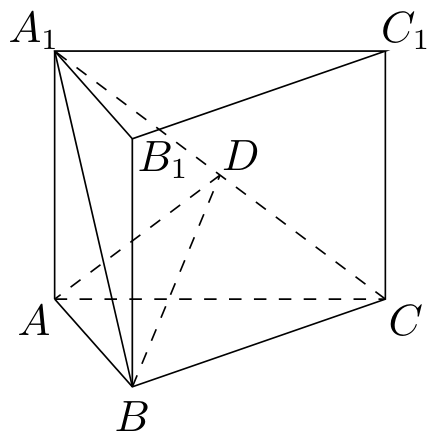
\includegraphics[width=4.3cm]{GaoKao/images/2022/new_gaokao_paper_1/q19_fig1.png}
\par}

        \begin{enumerate}[label=(\arabic*)]
            \item 求 $A$ 到平面 $A_1BC$ 的距离；
            \item 设 $D$ 为 $A_1C$ 的中点，$AA_1=AB$，平面 $A_1BC\perp$ 平面 $ABB_1A_1$，求二面角 $A$-$BD$-$C$ 的正弦值．
        \end{enumerate}

        \item （12分）

        一医疗团队为研究某地的一种地方性疾病与当地居民的卫生习惯（卫生习惯分为良好和不够良好两类）的关系，在已患该疾病的病例中随机调查了100例（称为病例组），同时在未患该疾病的人群中随机调查了100人（称为对照组），得到如下数据：

        \textsf{[插入表格：卫生习惯数据]}

        \begin{enumerate}[label=(\arabic*)]
            \item 能否有 $99\%$ 的把握认为患该疾病群体与未患该疾病群体的卫生习惯有差异？
            \item 从该地的人群中任选一人，$A$ 表示事件"选到的人卫生习惯不够良好"，$B$ 表示事件"选到的人患有该疾病"，$\dfrac{P(B\mid A)}{P(\bar{B}\mid A)}$ 与 $\dfrac{P(B\mid\bar{A})}{P(\bar{B}\mid\bar{A})}$ 的比值是卫生习惯不够良好对患该疾病风险程度的一项度量指标，记该指标为 $R$．
            \begin{enumerate}[label=(\roman*)]
                \item 证明：$R=\dfrac{P(A\mid B)}{P(\bar{A}\mid B)}\cdot\dfrac{P(\bar{A}\mid\bar{B})}{P(A\mid\bar{B})}$；
                \item 利用该调查数据，给出 $P(A\mid B),P(A\mid\bar{B})$ 的估计值，并利用（i）的结果给出 $R$ 的估计值．
            \end{enumerate}

            附：$K^2=\dfrac{n(ad-bc)^2}{(a+b)(c+d)(a+c)(b+d)}$，$P(K^2\geqslant k)$：0.050--3.841，0.010--6.635，0.001--10.828．
        \end{enumerate}

        \item （12分）

        已知点 $A(2,1)$ 在双曲线 $C:\dfrac{x^2}{a^2}-\dfrac{y^2}{a^2-1}=1\,(a>1)$ 上，直线 $l$ 交 $C$ 于 $P,Q$ 两点，直线 $AP,AQ$ 的斜率之和为 $0$．

        \begin{enumerate}[label=(\arabic*)]
            \item 求 $l$ 的斜率；
            \item 若 $\tan\angle PAQ=2\sqrt{2}$，求 $\triangle PAQ$ 的面积．
        \end{enumerate}

        \item （12分）

        已知函数 $f(x)=\mathrm{e}^x-ax$ 和 $g(x)=ax-\ln x$ 有相同的最小值．

        \begin{enumerate}[label=(\arabic*)]
            \item 求 $a$；
            \item 证明：存在直线 $y=b$，其与两条曲线 $y=f(x)$ 和 $y=g(x)$ 共有三个不同的交点，并且从左到右的三个交点的横坐标成等差数列．
        \end{enumerate}
    \end{enumerate}
\end{description}
\clearpage


\subsection{2022年新高考II卷}\label{gk:2022年新高考II卷}

\begin{description}
    \item[一、选择题] 本题共8小题，每小题5分，共40分．在每小题给出的四个选项中，只有一项是符合题目要求的．
    \begin{enumerate}[leftmargin=5pt]
        \item 已知集合 $A=\{-1,1,2,4\}$，$B=\{x\mid|x-1|\leqslant1\}$，则 $A\cap B=$
       
        {\centering\begin{tabular*}{\linewidth}{@{}@{\extracolsep{\fill}}llll@{}}
          \(\text{A. }\{-1,2\}\)  & \(\text{B. }\{1,2\}\)  & \(\text{C. }\{1,4\}\)  & \(\text{D. }\{-1,4\}\)
        \end{tabular*}\par}

        \item $(2+2\i)(1-2\i)=$
       
        {\centering\begin{tabular*}{\linewidth}{@{}@{\extracolsep{\fill}}llll@{}}
          \(\text{A. }-2+4\i\)  & \(\text{B. }-2-4\i\)  & \(\text{C. }6+2\i\)  & \(\text{D. }6-2\i\)
        \end{tabular*}\par}

        \item 图1是中国古代建筑中的举架结构，$AA',BB',CC',DD'$ 是桁，相邻桁的水平距离称为步，垂直距离称为举．图2是某古代建筑屋顶截面的示意图．其中 $DD_1,CC_1,BB_1,AA_1$ 是举，$OD_1,DC_1,CB_1,BA_1$ 是相等的步，相邻桁的举步之比分别为 $\dfrac{DD_1}{OD_1}=0.5$，$\dfrac{CC_1}{DC_1}=k_1$，$\dfrac{BB_1}{CB_1}=k_2$，$\dfrac{AA_1}{BA_1}=k_3$．已知 $k_1,k_2,k_3$ 成公差为 $0.1$ 的等差数列，且直线 $OA$ 的斜率为 $0.725$，则 $k_3=$
        
        {\centering
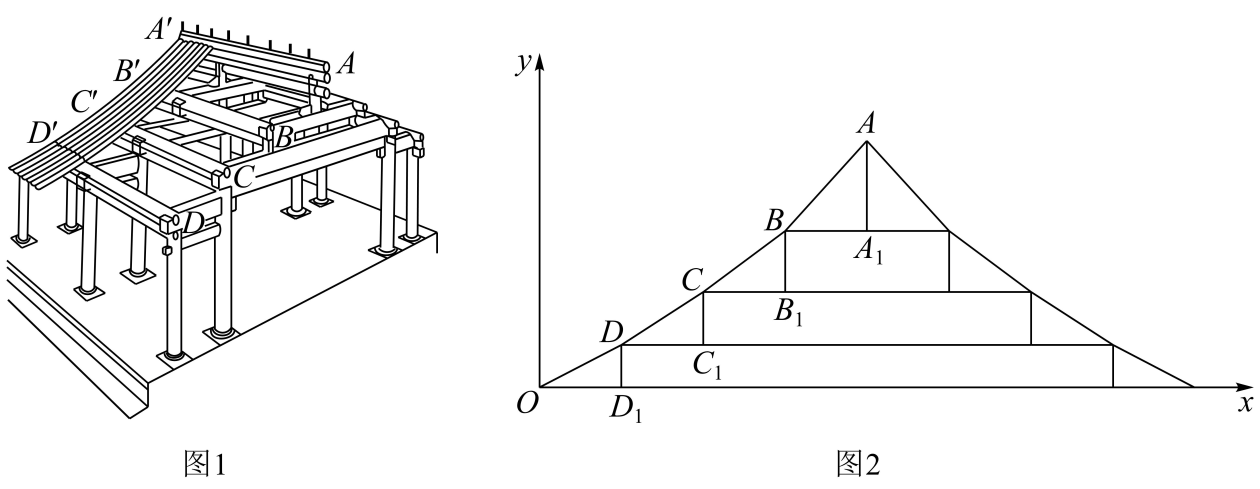
\includegraphics[width=16.0cm]{GaoKao/images/2022/new_gaokao_paper_2/q3_fig1.png}
\par}

        {\centering\begin{tabular*}{\linewidth}{@{}@{\extracolsep{\fill}}llll@{}}
          \(\text{A. }0.75\)  & \(\text{B. }0.8\)  & \(\text{C. }0.85\)  & \(\text{D. }0.9\)
        \end{tabular*}\par}

        \item 已知向量 $\bm a=(3,4)$，$\bm b=(1,0)$，$\bm c=\bm a+t\bm b$，若 $\langle\bm a,\bm c\rangle=\langle\bm b,\bm c\rangle$，则 $t=$
       
        {\centering\begin{tabular*}{\linewidth}{@{}@{\extracolsep{\fill}}llll@{}}
          \(\text{A. }-6\)  & \(\text{B. }-5\)  & \(\text{C. }5\)  & \(\text{D. }6\)
        \end{tabular*}\par}

        \item 甲、乙、丙、丁、戊5名同学站成一排参加文艺汇演，若甲不站在两端，丙和丁相邻，则不同的排列方式共有
       
        {\centering\begin{tabular*}{\linewidth}{@{}@{\extracolsep{\fill}}llll@{}}
          \(\text{A. }12\) 种  & \(\text{B. }24\) 种  & \(\text{C. }36\) 种  & \(\text{D. }48\) 种
        \end{tabular*}\par}

        \item 若 $\sin(\alpha+\beta)+\cos(\alpha+\beta)=2\sqrt{2}\cos\bigl(\alpha+\frac{\pi}{4}\bigr)\sin\beta$，则
       
        {\centering\begin{tabular*}{\linewidth}{@{}@{\extracolsep{\fill}}llll@{}}
          \(\text{A. }\tan(\alpha-\beta)=1\)  & \(\text{B. }\tan(\alpha+\beta)=1\)  & \(\text{C. }\tan(\alpha-\beta)=-1\)  & \(\text{D. }\tan(\alpha+\beta)=-1\)
        \end{tabular*}\par}

        \item 已知正三棱台的高为 $1$，上、下底面边长分别为 $3\sqrt{3}$ 和 $4\sqrt{3}$，其顶点都在同一球面上，则该球的表面积为
       
        {\centering\begin{tabular*}{\linewidth}{@{}@{\extracolsep{\fill}}llll@{}}
          \(\text{A. }100\pi\)  & \(\text{B. }128\pi\)  & \(\text{C. }144\pi\)  & \(\text{D. }192\pi\)
        \end{tabular*}\par}

        \item 若函数 $f(x)$ 的定义域为 $\mathbb{R}$，且 $f(x+y)+f(x-y)=f(x)f(y)$，$f(1)=1$，则 $\displaystyle\sum_{k=1}^{22}f(k)=$
       
        {\centering\begin{tabular*}{\linewidth}{@{}@{\extracolsep{\fill}}llll@{}}
          \(\text{A. }-3\)  & \(\text{B. }-2\)  & \(\text{C. }0\)  & \(\text{D. }1\)
        \end{tabular*}\par}
    \end{enumerate}
\end{description}

\begin{description}
    \item[二、选择题] 本题共4小题，每小题5分，共20分．在每小题给出的选项中，有多项符合题目要求．全部选对的得5分，部分选对的得2分，有选错的得0分．
    \begin{enumerate}[leftmargin=5pt]
      \addtocounter{enumi}{+8}
        \item 已知函数 $f(x)=\sin(2x+\varphi)\,(0<\varphi<\pi)$ 的图像关于点 $\bigl(\dfrac{2\pi}{3},0\bigr)$ 中心对称，则
        \begin{enumerate}[label=\Alph*.]
            \item $f(x)$ 在 $\bigl(0,\dfrac{5\pi}{12}\bigr)$ 单调递减
            \item $f(x)$ 在 $\bigl(-\dfrac{\pi}{12},\dfrac{11\pi}{12}\bigr)$ 有两个极值点
            \item 直线 $x=\dfrac{7\pi}{6}$ 是曲线 $y=f(x)$ 的对称轴
            \item 直线 $y=\dfrac{\sqrt{3}}{2}-x$ 是曲线 $y=f(x)$ 的切线
        \end{enumerate}

        \item 已知 $O$ 为坐标原点，过抛物线 $C:y^2=2px\,(p>0)$ 焦点 $F$ 的直线与 $C$ 交于 $A,B$ 两点，其中 $A$ 在第一象限，点 $M(p,0)$．若 $|AF|=|AM|$，则
        \begin{enumerate}[label=\Alph*.]
            \item 直线 $AB$ 的斜率为 $2\sqrt{6}$
            \item $|OB|=|OF|$
            \item $|AB|>4|OF|$
            \item $\angle OAM+\angle OBM<180^\circ$
        \end{enumerate}

        \item 如图，四边形 $ABCD$ 为正方形，$ED\perp$ 平面 $ABCD$，$FB\parallel ED$，$AB=ED=2FB$．记三棱锥 $E$-$ACD$，$F$-$ABC$，$F$-$ACE$ 的体积分别为 $V_1,V_2,V_3$，则
        
        {\centering
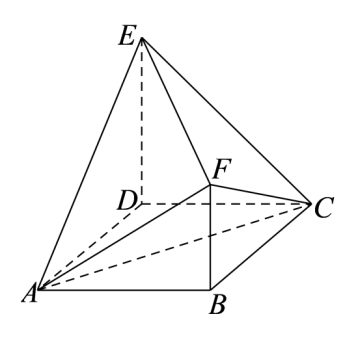
\includegraphics[width=6.0cm]{GaoKao/images/2022/new_gaokao_paper_2/q11_fig1.png}
\par}

        \begin{enumerate}[label=\Alph*.]
            \item $V_3=2V_2$
            \item $V_3=V_1$
            \item $V_3=V_1+V_2$
            \item $2V_3=3V_1$
        \end{enumerate}

        \item 若 $x,y$ 满足 $x^2+y^2-xy=1$，则
        \begin{enumerate}[label=\Alph*.]
            \item $x+y\leqslant1$
            \item $x+y\geqslant-2$
            \item $x^2+y^2\leqslant2$
            \item $x^2+y^2\geqslant1$
        \end{enumerate}
    \end{enumerate}
\end{description}

\begin{description}
    \item[三、填空题] 本题共4小题，每小题5分，共20分．
    \begin{enumerate}[leftmargin=5pt]
      \addtocounter{enumi}{+12}
        \item 已知随机变量 $X$ 服从正态分布 $N(2,\sigma^2)$，且 $P(2<X\leqslant2.5)=0.36$，则 $P(X>2.5)=$ \rule[-0.3ex]{3em}{0.4pt}．
        \item 曲线 $y=\ln|x|$ 过坐标原点的两条切线的方程为 \rule[-0.3ex]{3em}{0.4pt}，\rule[-0.3ex]{3em}{0.4pt}．
        \item 设点 $A(-2,3)$，$B(0,a)$，若直线 $AB$ 关于 $y=a$ 对称的直线与圆 $(x+3)^2+(y+2)^2=1$ 有公共点，则 $a$ 的取值范围是 \rule[-0.3ex]{3em}{0.4pt}．
        \item 已知直线 $l$ 与椭圆 $\dfrac{x^2}{6}+\dfrac{y^2}{3}=1$ 在第一象限交于 $A,B$ 两点，$l$ 与 $x$ 轴、$y$ 轴分别交于 $M,N$ 两点，且 $|MA|=|NB|$，$|MN|=2\sqrt{3}$，则 $l$ 的方程为 \rule[-0.3ex]{3em}{0.4pt}．
    \end{enumerate}
\end{description}

\begin{description}
    \item[四、解答题] 本题共6小题，共70分．解答应写出文字说明、证明过程或演算步骤．
    \begin{enumerate}[leftmargin=5pt]
      \addtocounter{enumi}{+16}
        \item （10分）

        已知 $\{a_n\}$ 为等差数列，$\{b_n\}$ 是公比为 $2$ 的等比数列，且 $a_2-b_2=a_3-b_3=b_4-a_4$．

        \begin{enumerate}[label=(\arabic*)]
            \item 证明：$a_1=b_1$；
            \item 求集合 $\{k\mid b_k=a_m+a_1,1\leqslant m\leqslant500\}$ 中元素的个数．
        \end{enumerate}

        \item （12分）

        记 $\triangle ABC$ 的内角 $A,B,C$ 的对边分别为 $a,b,c$，分别以 $a,b,c$ 为边长的三个正三角形的面积依次为 $S_1,S_2,S_3$．已知 $S_1-S_2+S_3=\dfrac{\sqrt{3}}{2}$，$\sin B=\dfrac{1}{3}$．

        \begin{enumerate}[label=(\arabic*)]
            \item 求 $\triangle ABC$ 的面积；
            \item 若 $\sin A\sin C=\dfrac{\sqrt{2}}{3}$，求 $b$．
        \end{enumerate}

        \item （12分）

        在某地区进行流行病学调查，随机调查了100位某种疾病患者的年龄，得到如下的样本数据的频率分布直方图：

        {\centering
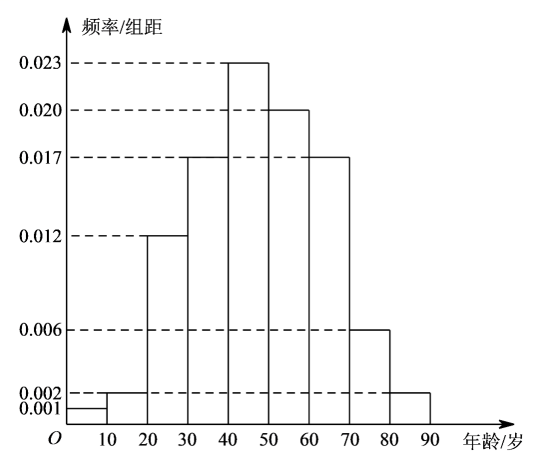
\includegraphics[width=0.65\linewidth]{GaoKao/images/2022/new_gaokao_paper_2/q19_fig1.png}
\par}

        \begin{enumerate}[label=(\arabic*)]
            \item 估计该地区这种疾病患者的平均年龄（同一组数据用该组区间的中点值为代表）；
            \item 估计该地区一位这种疾病患者的年龄位于区间$[20,70)$的概率；
            \item 已知该地区这种疾病患者的患病率为$0.1\%$，该地区年龄位于区间$[40,50)$的人口占该地区总人口的$16\%$．从该地区中任选一人，若此人的年龄位于区间$[40,50)$，求此人患这种疾病的概率（以样本数据中患者的年龄位于各区间的频率作为患者的年龄位于该区间的概率，精确到0.0001）．
        \end{enumerate}

        \item （12分）

        如图，$PO$ 是三棱锥 $P$-$ABC$ 的高，$PA=PB$，$AB\perp AC$，$E$ 为 $PB$ 的中点．

        {\centering
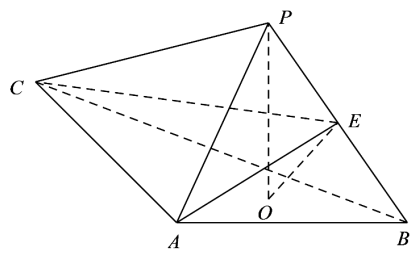
\includegraphics[width=10.9cm]{GaoKao/images/2022/new_gaokao_paper_2/q20_fig1.png}
\par}

        \begin{enumerate}[label=(\arabic*)]
            \item 证明：$OE\parallel$ 平面 $PAC$；
            \item 若 $\angle ABO=\angle CBO=30^\circ$，$PO=3$，$PA=5$，求二面角 $C$-$AE$-$B$ 的正弦值．
        \end{enumerate}

        \item （12分）

        已知双曲线 $C:\dfrac{x^2}{a^2}-\dfrac{y^2}{b^2}=1\,(a>0,b>0)$ 的右焦点为 $F(2,0)$，渐近线方程为 $y=\pm\sqrt{3}x$．

        \begin{enumerate}[label=(\arabic*)]
            \item 求 $C$ 的方程；
            \item 过 $F$ 的直线与 $C$ 的两条渐近线分别交于 $A,B$ 两点，点 $P(x_1,y_1),Q(x_2,y_2)$ 在 $C$ 上，且 $x_1>x_2>0$，$y_1>0$．过 $P$ 且斜率为 $-\sqrt{3}$ 的直线与过 $Q$ 且斜率为 $\sqrt{3}$ 的直线交于点 $M$．从下面\ding{172}\ding{173}\ding{174}中选取两个作为条件，证明另外一个成立．
            \begin{quote}
            \ding{172}$M$ 在 $AB$ 上；\ding{173}$PQ\parallel AB$；\ding{174}$|MA|=|MB|$．
            \end{quote}
            注：若选择不同的组合分别解答，则按第一个解答计分．
        \end{enumerate}

        \item （12分）

        已知函数 $f(x)=x\mathrm{e}^{ax}-\mathrm{e}^x$．

        \begin{enumerate}[label=(\arabic*)]
            \item 当 $a=1$ 时，讨论 $f(x)$ 的单调性；
            \item 当 $x>0$ 时，$f(x)<-1$，求 $a$ 的取值范围；
            \item 设 $n\in\mathbb{N}^*$，证明：$\dfrac{1}{\sqrt{1^2+1}}+\dfrac{1}{\sqrt{2^2+2}}+\cdots+\dfrac{1}{\sqrt{n^2+n}}>\ln(n+1)$．
        \end{enumerate}
    \end{enumerate}
\end{description}
\clearpage


\subsection{2022年北京卷}\label{gk:2022年北京卷}

\begin{description}
    \item[一、选择题] 本题共10小题，每小题4分，共40分．在每小题给出的四个选项中，选出符合题目要求的一项．
    \begin{enumerate}[leftmargin=5pt]
        \item 已知全集 $U=\{x\mid -3<x<3\}$，集合 $A=\{x\mid -2<x\leqslant1\}$，则 $\complement_U A=$
       
        {\centering\begin{tabular*}{\linewidth}{@{}@{\extracolsep{\fill}}llll@{}}
          \(\text{A. }(-2,1]\)  & \(\text{B. }(-3,-2)\cup[1,3)\)  & \(\text{C. }[-2,1)\)  & \(\text{D. }(-3,-2]\cup(1,3)\)
        \end{tabular*}\par}

        \item 若复数 $z$ 满足 $\i z=3-4\i$，则 $|z|=$
       
        {\centering\begin{tabular*}{\linewidth}{@{}@{\extracolsep{\fill}}llll@{}}
          \(\text{A. }1\)  & \(\text{B. }5\)  & \(\text{C. }7\)  & \(\text{D. }25\)
        \end{tabular*}\par}

        \item 若直线 $2x+y-1=0$ 是圆 $(x-a)^2+y^2=1$ 的一条对称轴，则 $a=$
       
        {\centering\begin{tabular*}{\linewidth}{@{}@{\extracolsep{\fill}}llll@{}}
          \(\text{A. }\dfrac{1}{2}\)  & \(\text{B. }-\dfrac{1}{2}\)  & \(\text{C. }1\)  & \(\text{D. }-1\)
        \end{tabular*}\par}

        \item 已知函数 $f(x)=\dfrac{1}{1+2^x}$，则对任意实数 $x$，有
       
        {\centering\begin{tabular*}{\linewidth}{@{}@{\extracolsep{\fill}}llll@{}}
          \(\text{A. }f(-x)+f(x)=0\)  & \(\text{B. }f(-x)-f(x)=0\)  & \(\text{C. }f(-x)+f(x)=1\)  & \(\text{D. }f(-x)-f(x)=\dfrac{1}{3}\)
        \end{tabular*}\par}

        \item 已知函数 $f(x)=\cos^2 x-\sin^2 x$，则
       
        {\centering\begin{tabular*}{\linewidth}{@{}@{\extracolsep{\fill}}llll@{}}
          \(\text{A. }f(x)$ 在 $\bigl(-\dfrac{\pi}{2},-\dfrac{\pi}{6}\bigr)$ 上单调递减  & \(\text{B. }f(x)$ 在 $\bigl(-\dfrac{\pi}{4},\dfrac{\pi}{12}\bigr)$ 上单调递增 \\
          \(\text{C. }f(x)$ 在 $\bigl(0,\dfrac{\pi}{3}\bigr)$ 上单调递减  & \(\text{D. }f(x)$ 在 $\bigl(\dfrac{\pi}{4},\dfrac{7\pi}{12}\bigr)$ 上单调递增
        \end{tabular*}\par}

        \item 设 $\{a_n\}$ 是公差不为0的无穷等差数列，则"$\{a_n\}$ 为递增数列"是"存在正整数 $N_0$，当 $n>N_0$ 时，$a_n>0$"的
       
        {\centering\begin{tabular*}{\linewidth}{@{}@{\extracolsep{\fill}}llll@{}}
          \(\text{A. }\)充分不必要条件  & \(\text{B. }\)必要不充分条件  & \(\text{C. }\)充要条件  & \(\text{D. }\)既不充分也不必要条件
        \end{tabular*}\par}

        \item 在北京冬奥会上，国家速滑馆"冰丝带"使用高效环保的二氧化碳跨临界直冷制冰技术，为实现绿色冬奥作出了贡献．如图描述了一定条件下二氧化碳所处的状态与 $T$ 和 $\lg P$ 的关系，其中 $T$ 表示温度，单位是 $\text{K}$；$P$ 表示压强，单位是 $\text{bar}$．下列结论中正确的是
        
        {\centering
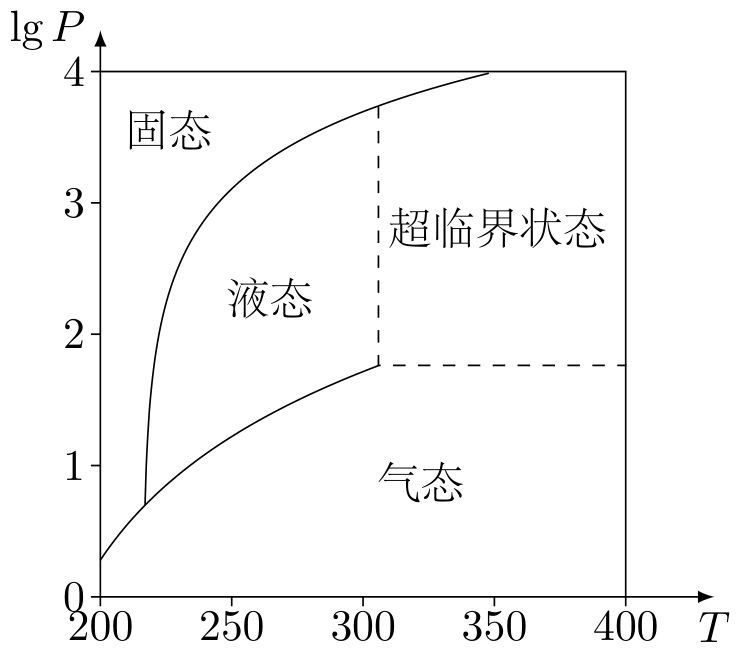
\includegraphics[width=7.1cm]{GaoKao/images/2022/beijing/q7_fig1.png}
\par}

        {\centering\begin{tabular*}{\linewidth}{@{}@{\extracolsep{\fill}}llll@{}}
          \(\text{A. }\)当 $T=220$，$P=1026$ 时，二氧化碳处于液态 \\
          \(\text{B. }\)当 $T=270$，$P=128$ 时，二氧化碳处于气态 \\
          \(\text{C. }\)当 $T=300$，$P=9987$ 时，二氧化碳处于超临界状态 \\
          \(\text{D. }\)当 $T=360$，$P=729$ 时，二氧化碳处于超临界状态
        \end{tabular*}\par}

        \item 若 $(2x-1)^4=a_4x^4+a_3x^3+a_2x^2+a_1x+a_0$，则 $a_0+a_2+a_4=$
       
        {\centering\begin{tabular*}{\linewidth}{@{}@{\extracolsep{\fill}}llll@{}}
          \(\text{A. }40\)  & \(\text{B. }41\)  & \(\text{C. }-40\)  & \(\text{D. }-41\)
        \end{tabular*}\par}

        \item 已知正三棱锥 $P$-$ABC$ 的六条棱长均为 $6$，$S$ 是 $\triangle ABC$ 及其内部的点构成的集合．设集合 $T=\{Q\in S\mid PQ\leqslant5\}$，则 $T$ 表示的区域的面积为
       
        {\centering\begin{tabular*}{\linewidth}{@{}@{\extracolsep{\fill}}llll@{}}
          \(\text{A. }\dfrac{3\pi}{4}\)  & \(\text{B. }\pi\)  & \(\text{C. }2\pi\)  & \(\text{D. }3\pi\)
        \end{tabular*}\par}

        \item 在 $\triangle ABC$ 中，$AC=3$，$BC=4$，$\angle C=90^\circ$．$P$ 为 $\triangle ABC$ 所在平面内的动点，且 $PC=1$，则 $\overrightarrow{PA}\cdot\overrightarrow{PB}$ 的取值范围是
       
        {\centering\begin{tabular*}{\linewidth}{@{}@{\extracolsep{\fill}}llll@{}}
          \(\text{A. }[-5,3]\)  & \(\text{B. }[-3,5]\)  & \(\text{C. }[-6,4]\)  & \(\text{D. }[-4,6]\)
        \end{tabular*}\par}
    \end{enumerate}
\end{description}

\begin{description}
    \item[二、填空题] 本题共5小题，每小题5分，共25分．
    \begin{enumerate}[leftmargin=5pt]
      \addtocounter{enumi}{+10}
        \item 函数 $f(x)=\dfrac{1}{x}+\sqrt{1-x}$ 的定义域是 \rule[-0.3ex]{3em}{0.4pt}．
        \item 已知双曲线 $y^2+\dfrac{x^2}{m}=1$ 的渐近线方程为 $y=\pm\dfrac{\sqrt{3}}{3}x$，则 $m=$ \rule[-0.3ex]{3em}{0.4pt}．
        \item 若函数 $f(x)=A\sin x-\sqrt{3}\cos x$ 的一个零点为 $\dfrac{\pi}{3}$，则 $A=$ \rule[-0.3ex]{3em}{0.4pt}；$f\bigl(\dfrac{\pi}{12}\bigr)=$ \rule[-0.3ex]{3em}{0.4pt}．
        \item 设函数 $f(x)=\begin{cases}-ax+1,&x<a,\\(x-2)^2,&x\geqslant a.\end{cases}$ 若 $f(x)$ 存在最小值，则 $a$ 的一个取值为 \rule[-0.3ex]{3em}{0.4pt}；$a$ 的最大值为 \rule[-0.3ex]{3em}{0.4pt}．
        \item 已知数列 $\{a_n\}$ 的各项均为正数，其前 $n$ 项和 $S_n$ 满足 $a_n\cdot S_n=9\,(n=1,2,\cdots)$．给出下列四个结论：

        \ding{172}$\{a_n\}$ 的第2项小于3；
        \ding{173}$\{a_n\}$ 为等比数列；
        \ding{174}$\{a_n\}$ 为递减数列；
        \ding{175}$\{a_n\}$ 中存在小于 $\dfrac{1}{100}$ 的项．

        其中所有正确结论的序号是 \rule[-0.3ex]{3em}{0.4pt}．
    \end{enumerate}
\end{description}

\begin{description}
    \item[三、解答题] 本题共6小题，共85分．解答应写出文字说明、证明过程或演算步骤．
    \begin{enumerate}[leftmargin=5pt]
      \addtocounter{enumi}{+15}
        \item （13分）

        在 $\triangle ABC$ 中，$\sin2C=\sqrt{3}\sin C$．

        \begin{enumerate}[label=(\arabic*)]
            \item 求 $\angle C$；
            \item 若 $b=6$，且 $\triangle ABC$ 的面积为 $6\sqrt{3}$，求 $\triangle ABC$ 的周长．
        \end{enumerate}

        \item （14分）

        如图，在三棱柱 $ABC$-$A_1B_1C_1$ 中，侧面 $BCC_1B_1$ 为正方形，平面 $BCC_1B_1\perp$ 平面 $ABB_1A_1$，$AB=BC=2$，$M,N$ 分别为 $A_1B_1,AC$ 的中点．

        {\centering
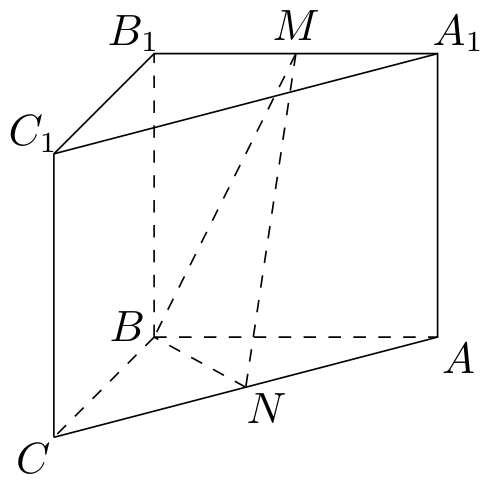
\includegraphics[width=5.1cm]{GaoKao/images/2022/beijing/q17_fig1.png}
\par}

        \begin{enumerate}[label=(\arabic*)]
            \item 求证：$MN\parallel$ 平面 $BCC_1B_1$；
            \item 再从条件\ding{172}、条件\ding{173}中选择一个作为已知，求直线 $AB$ 与平面 $BMN$ 所成角的正弦值．
            \begin{quote}
            条件\ding{172}：$AB\perp MN$；条件\ding{173}：$BM=MN$．
            \end{quote}
        \end{enumerate}

        \item （14分）

        在校运动会上，只有甲、乙、丙三名同学参加铅球比赛，比赛成绩达到 $9.50\,\text{m}$ 以上（含 $9.50\,\text{m}$）的同学将获得优秀奖．为预测获得优秀奖的人数及冠军得主，收集了甲、乙、丙以往的比赛成绩，并整理得到如下数据（单位：m）：

        甲：$9.80,9.70,9.55,9.54,9.48,9.42,9.40,9.35,9.30,9.25$；

        乙：$9.78,9.56,9.51,9.36,9.32,9.23$；

        丙：$9.85,9.65,9.20,9.16$．

        假设用频率估计概率，且甲、乙、丙的比赛成绩相互独立．

        \begin{enumerate}[label=(\arabic*)]
            \item 估计甲在校运动会铅球比赛中获得优秀奖的概率；
            \item 设 $X$ 是甲、乙、丙在校运动会铅球比赛中获得优秀奖的总人数，估计 $X$ 的数学期望 $EX$；
            \item 在校运动会铅球比赛中，甲、乙、丙谁获得冠军的概率估计值最大？（结论不要求证明）
        \end{enumerate}

        \item （15分）

        已知椭圆 $E:\dfrac{x^2}{a^2}+\dfrac{y^2}{b^2}=1\,(a>b>0)$ 的一个顶点为 $A(0,1)$，焦距为 $2\sqrt{3}$．

        \begin{enumerate}[label=(\arabic*)]
            \item 求椭圆 $E$ 的方程；
            \item 过点 $P(-2,1)$ 作斜率为 $k$ 的直线与椭圆 $E$ 交于不同的两点 $B,C$，直线 $AB,AC$ 分别与 $x$ 轴交于点 $M,N$．当 $|MN|=2$ 时，求 $k$ 的值．
        \end{enumerate}

        \item （15分）

        已知函数 $f(x)=\mathrm{e}^x\ln(1+x)$．

        \begin{enumerate}[label=(\arabic*)]
            \item 求曲线 $y=f(x)$ 在点 $(0,f(0))$ 处的切线方程；
            \item 设 $g(x)=f'(x)$，讨论函数 $g(x)$ 在 $[0,+\infty)$ 上的单调性；
            \item 证明：对任意的 $s,t\in(0,+\infty)$，有 $f(s+t)>f(s)+f(t)$．
        \end{enumerate}

        \item （15分）

        已知 $Q:a_1,a_2,\cdots,a_k$ 为有穷整数数列．给定正整数 $m$，若对任意的 $n\in\{1,2,\cdots,m\}$，在 $Q$ 中存在 $a_i,a_{i+1},\cdots,a_{i+j}\,(j\geqslant0)$，使得 $a_i+a_{i+1}+\cdots+a_{i+j}=n$，则称 $Q$ 为 $m$-连续可表数列．

        \begin{enumerate}[label=(\arabic*)]
            \item 判断 $Q:2,1,4$ 是否为 $5$-连续可表数列？是否为 $6$-连续可表数列？说明理由；
            \item 若 $Q:a_1,a_2,\cdots,a_8$ 为 $8$-连续可表数列，求证：$k$ 的最小值为 $4$；
            \item 若 $Q:a_1,a_2,\cdots,a_4$ 为 $20$-连续可表数列，且 $a_1+a_2+a_3+a_4<20$，求证：$k\geqslant7$．
        \end{enumerate}
    \end{enumerate}
\end{description}
\clearpage


\subsection{2022年上海卷}\label{gk:2022年上海卷}

\begin{description}
    \item[一、填空题] 本大题共有12题，满分54分，第1\textasciitilde6题每题4分，第7\textasciitilde12题每题5分．
    \begin{enumerate}[leftmargin=5pt]
        \item 已知 $z=1+\i$，则 $\bar{z}=$ \rule[-0.3ex]{3em}{0.4pt}．
        \item 双曲线 $\dfrac{x^2}{9}-y^2=1$ 的实轴长为 \rule[-0.3ex]{3em}{0.4pt}．
        \item 函数 $f(x)=\cos^2 x-\sin^2 x+1$ 的周期为 \rule[-0.3ex]{3em}{0.4pt}．
        \item 已知 $a\in\mathbb{R}$，行列式 $\begin{vmatrix}a&1\\3&2\end{vmatrix}$ 的值与行列式 $\begin{vmatrix}a&3\\6&a\end{vmatrix}$ 的值相等，则 $a=$ \rule[-0.3ex]{3em}{0.4pt}．
        \item 已知圆柱的高为 $4$，底面积为 $9\pi$，则圆柱的侧面积为 \rule[-0.3ex]{3em}{0.4pt}．
        \item 已知 $x-y=1$，则 $x^2+y^2$ 的最小值为 \rule[-0.3ex]{3em}{0.4pt}．
        \item 二项式 $(3x+1)^n$ 的展开式中，$x^2$ 的系数是 $x$ 的系数的 $4$ 倍，则 $n=$ \rule[-0.3ex]{3em}{0.4pt}．
        \item 若函数 $f(x)=\begin{cases}a^x,&x<0,\\x+a,&x\geqslant0,\end{cases}$ 为奇函数，则 $a=$ \rule[-0.3ex]{3em}{0.4pt}．
        \item 为了检测学生的身体素质指标，从游泳类，球类，田径类三个大项中随机选取4项作为测试项目，若每类至少有一个项目，则不同的选取方式有 \rule[-0.3ex]{3em}{0.4pt} 种（用数字作答）．
        \item 已知等差数列 $\{a_n\}$ 的公差不为零，$S_n$ 为其前 $n$ 项和，若 $S_5=0$，则 $S_i\,(i=0,1,2,\cdots,100)$ 中不同的数值有 \rule[-0.3ex]{3em}{0.4pt} 个．
        \item 已知 $\lambda>0$，平面向量 $\overrightarrow{OA},\overrightarrow{OB}$ 满足 $|\overrightarrow{OA}|=1$，$|\overrightarrow{OA}+2\overrightarrow{OB}|=\lambda|\overrightarrow{OA}-2\overrightarrow{OB}|$，$\overrightarrow{OA}\cdot\overrightarrow{OB}=0$，$\overrightarrow{OP}=\lambda\overrightarrow{OA}+\mu\overrightarrow{OB}$，其中 $\lambda,\mu>0$ 且 $\lambda+\mu=2$，则 $|\overrightarrow{OP}|$ 的最小值为 \rule[-0.3ex]{3em}{0.4pt}．
        \item 设函数 $f(x)$ 满足 $f(x)=f(|x-1|)$，对任意 $x_1,x_2\in[0,+\infty)$，均有 $f(x_1)-f(x_2)=f(x_1+x_2)$，则 $f(x)$ 在 $(0,1)$ 上的解析式为 \rule[-0.3ex]{3em}{0.4pt}．
    \end{enumerate}
\end{description}

\begin{description}
    \item[二、选择题] 本题共4小题，每小题5分，共20分．
    \begin{enumerate}[leftmargin=5pt]
      \addtocounter{enumi}{+12}
        \item 若实数 $a,b$ 满足 $a>b>0$，下列不等式中恒成立的是
       
        {\centering\begin{tabular*}{\linewidth}{@{}@{\extracolsep{\fill}}llll@{}}
          \(\text{A. }a+b>2\sqrt{ab}\)  & \(\text{B. }a+b<2\sqrt{ab}\)  & \(\text{C. }\dfrac{a}{2}+2b>2\sqrt{ab}\)  & \(\text{D. }\dfrac{a}{2}+2b<2\sqrt{ab}\)
        \end{tabular*}\par}

        \item 为比较甲、乙两地某月14时的气温情况，随机选取该月中的5天，将这5天中14时的气温数据（单位：$^\circ\text{C}$）制成如图所示的茎叶图，考虑以下结论：
        
        \textsf{[插入图片：茎叶图]}

        \ding{172}甲地该月14时的平均气温低于乙地该月14时的平均气温；
        \ding{173}甲地该月14时的平均气温高于乙地该月14时的平均气温；
        \ding{174}甲地该月14时的气温的标准差小于乙地该月14时的气温的标准差；
        \ding{175}甲地该月14时的气温的标准差大于乙地该月14时的气温的标准差．

        其中根据茎叶图能得到的统计结论的编号为
       
        {\centering\begin{tabular*}{\linewidth}{@{}@{\extracolsep{\fill}}llll@{}}
          \(\text{A. }\)\ding{172}\ding{174}  & \(\text{B. }\)\ding{172}\ding{175}  & \(\text{C. }\)\ding{173}\ding{174}  & \(\text{D. }\)\ding{173}\ding{175}
        \end{tabular*}\par}

        \item 如图，正方体 $ABCD$-$A_1B_1C_1D_1$ 中，$P,Q,R,S$ 分别为棱 $AB,BC,BB_1,CD$ 的中点，连接 $PQ,A_1S,B_1R$．对空间任意两点 $M,N$，若线段 $MN$ 上不存在点在线段 $PQ,A_1S,B_1R$ 上，则称 $M,N$ 两点可视．则下列选项中与点 $D_1$ 可视的点为
        
        {\centering
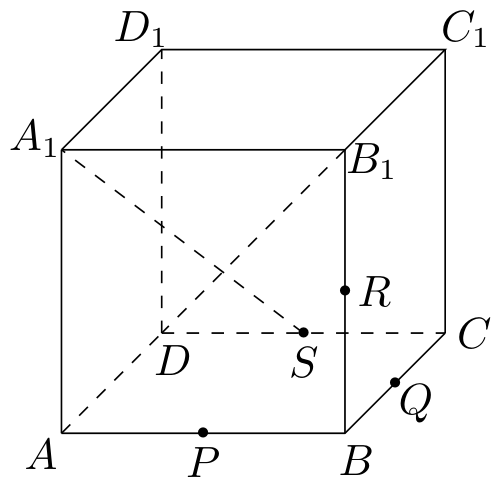
\includegraphics[width=5.1cm]{GaoKao/images/2022/shanghai/q15_fig1.png}
\par}

        {\centering\begin{tabular*}{\linewidth}{@{}@{\extracolsep{\fill}}llll@{}}
          \(\text{A. }\)点 $P$  & \(\text{B. }\)点 $B$  & \(\text{C. }\)点 $R$  & \(\text{D. }\)点 $Q$
        \end{tabular*}\par}

        \item 已知 $a_1,a_2,\cdots,a_k$ 是 $1,2,\cdots,k$ 的一个排列，设 $S=a_1+2a_2+\cdots+ka_k$，则 $S$ 的最大值与最小值的差为
       
        {\centering\begin{tabular*}{\linewidth}{@{}@{\extracolsep{\fill}}llll@{}}
          \(\text{A. }\dfrac{k^3+k^2-2k}{3}\)  & \(\text{B. }\dfrac{k^3+k^2-2}{3}\)  & \(\text{C. }\dfrac{k^3-k^2-2k}{3}\)  & \(\text{D. }\dfrac{k^3-k}{2}\)
        \end{tabular*}\par}
    \end{enumerate}
\end{description}

\begin{description}
    \item[三、解答题] 本题共5小题，共76分．
    \begin{enumerate}[leftmargin=5pt]
      \addtocounter{enumi}{+16}
        \item （14分）

        如图，$AD=BC=6$，$AB=20$，$\angle DAB=\angle ABC=120^\circ$，$O$ 为 $AB$ 中点，曲线 $CD$ 上任意一点到点 $O$ 的距离均相等，$P,M,Q$ 为曲线 $CD$ 上的点，且 $MO\perp AB$，点 $P$ 与点 $Q$ 关于直线 $OM$ 对称．

        {\centering
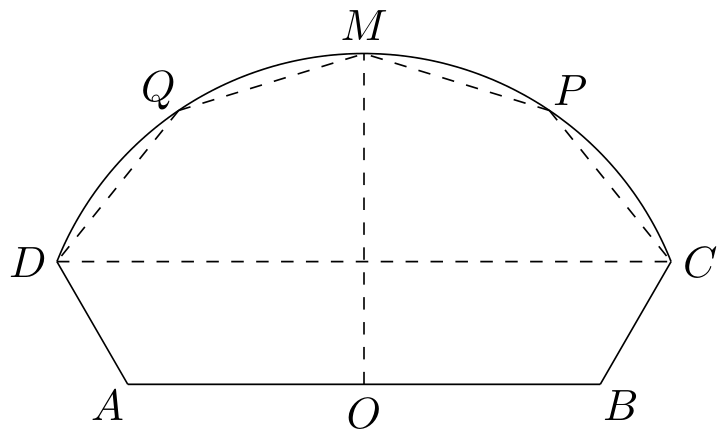
\includegraphics[width=8.7cm]{GaoKao/images/2022/shanghai/q19_fig1.png}
\par}

        \begin{enumerate}[label=(\arabic*)]
            \item 若点 $P$ 在曲线 $CD$ 上，且点 $P$ 与点 $C$ 的距离等于点 $P$ 与点 $D$ 的距离，求点 $P$ 的位置；
            \item 求五边形 $MOABQ$ 的面积的最大值．
        \end{enumerate}

        \item （14分）

        已知函数 $f(x)=\log_3(a+x)+\log_3(6-x)$．

        \begin{enumerate}[label=(\arabic*)]
            \item 若将函数 $f(x)$ 的图像向下平移 $m\,(m>0)$ 个单位后，经过点 $(3,0)$ 与 $(5,0)$，求 $a$ 与 $m$ 的值；
            \item 若 $a>-3$ 且 $a\neq0$，求解不等式 $f(x)\leqslant f(6-x)$．
        \end{enumerate}

        \item （14分）

        如图，为保护河上古桥 $OA$，规划建一座新桥 $BC$，同时设立一个圆形保护区．规划要求：新桥 $BC$ 与河岸 $AB$ 垂直；保护区的边界为圆心 $M$ 在线段 $OA$ 上并与 $BC$ 相切的圆，且古桥两端 $O$ 和 $A$ 到该圆上任意一点的距离均不少于 $80\,\text{m}$．经测量，点 $A$ 位于点 $O$ 正北方向 $60\,\text{m}$ 处，点 $C$ 位于点 $O$ 正东方向 $170\,\text{m}$ 处（$OC$ 为河岸），$\tan\angle BCO=\dfrac{4}{3}$．

        \textsf{[插入图片：河岸桥梁示意图]}

        \begin{enumerate}[label=(\arabic*)]
            \item 求新桥 $BC$ 的长；
            \item 当 $OM$ 多长时，圆形保护区的面积最大？
        \end{enumerate}

        \item （17分）

        已知椭圆 $\Gamma:\dfrac{x^2}{a^2}+\dfrac{y^2}{b^2}=1\,(a>b>0)$，点 $A(0,-2)$，椭圆 $\Gamma$ 经过点 $A$ 且离心率 $e=\dfrac{\sqrt{3}}{2}$．过点 $B(1,0)$ 的直线 $l$ 交椭圆于 $M,N$ 两点（点 $M$ 在 $x$ 轴上方），点 $P$ 为 $y$ 轴上一点，且 $PM=PN$，点 $P$ 的纵坐标为 $t$．

        \begin{enumerate}[label=(\arabic*)]
            \item 求椭圆 $\Gamma$ 的标准方程；
            \item 若点 $P$ 的坐标为 $(0,1)$，求直线 $l$ 的方程；
            \item 若存在直线 $l$ 使得 $|PM|=|PN|=|MN|$，求 $t$ 的取值范围．
        \end{enumerate}

        \item （17分）

        已知函数 $f(x)$ 的定义域为 $\mathbb{R}$，现有下面两种对 $f(x)$ 的变换：

        $\omega$：$f(x)\to f(x+t)-f(x)$，其中 $t$ 为常数；

        $\sigma$：$f(x)\to f(x)+f(-x)$．

        \begin{enumerate}[label=(\arabic*)]
            \item 若 $f(x)=2^x$，$t=1$，对 $f(x)$ 进行 $\omega$ 变换后得到函数 $g(x)$，求方程 $g(x)=2$ 的解；
            \item 若 $f(x)=x^2$，对 $f(x)$ 进行 $\omega$ 变换后得到函数 $h(x)$，解不等式 $f(x)\geqslant h(x)+2$；
            \item 已知 $f(x)$ 是在 $\mathbb{R}$ 上单调递增的奇函数，$f(-1)=0$，先对 $f(x)$ 进行 $\sigma$ 变换后得到 $u(x)$，再对 $u(x)$ 进行 $\omega$ 变换后得到 $h_1(x)$；先对 $f(x)$ 进行 $\omega$ 变换后得到 $v(x)$，再对 $v(x)$ 进行 $\sigma$ 变换后得到 $h_2(x)$．若 $h_1(x)=h_2(x)$ 对任意 $t$ 成立，证明：$f(x)$ 是线性函数．
        \end{enumerate}
    \end{enumerate}
\end{description}
\clearpage


\subsection{2022年天津卷}\label{gk:2022年天津卷}

\begin{description}
    \item[一、选择题] 本题共9小题，每小题5分，共45分．在每小题给出的四个选项中，只有一项是符合题目要求的．
    \begin{enumerate}[leftmargin=5pt]
        \item 设全集 $U=\{-2,-1,0,1,2\}$，集合 $A=\{0,1,2\}$，$B=\{-1,2\}$，则 $A\cap\complement_U B=$
       
        {\centering\begin{tabular*}{\linewidth}{@{}@{\extracolsep{\fill}}llll@{}}
          \(\text{A. }\{0,1\}\)  & \(\text{B. }\{0,1,2\}\)  & \(\text{C. }\{-1,1,2\}\)  & \(\text{D. }\{0,-1,1,2\}\)
        \end{tabular*}\par}

        \item "$x$ 为整数"是"$2x+1$ 为整数"的
       
        {\centering\begin{tabular*}{\linewidth}{@{}@{\extracolsep{\fill}}llll@{}}
          \(\text{A. }\)充分不必要条件  & \(\text{B. }\)必要不充分条件  & \(\text{C. }\)充要条件  & \(\text{D. }\)既不充分也不必要条件
        \end{tabular*}\par}

        \item 函数 $f(x)=\dfrac{|x^2-1|}{x}$ 的图像为
        
        {\centering
            \begin{tabular*}{\linewidth}{@{}@{\extracolsep{\fill}}cccc@{}}
            \(\text{A. }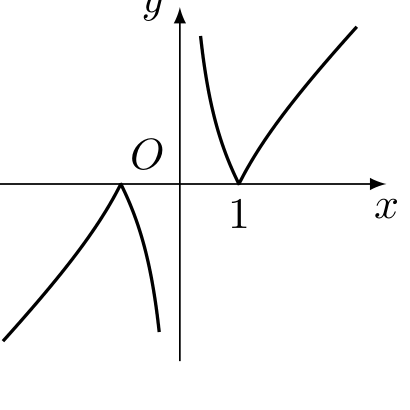
\includegraphics[width=0.15\paperwidth]{GaoKao/images/2022/tianjin/q3_option_a.png}\)  &  \(\text{B. }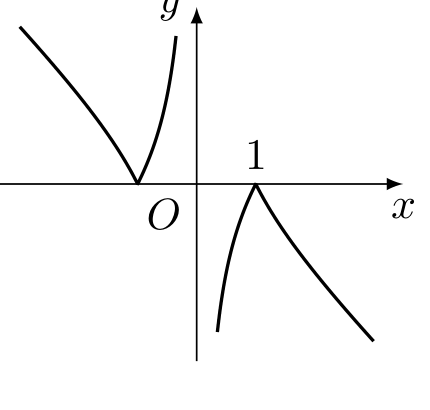
\includegraphics[width=0.15\paperwidth]{GaoKao/images/2022/tianjin/q3_option_b.png}\)  &  \(\text{C. }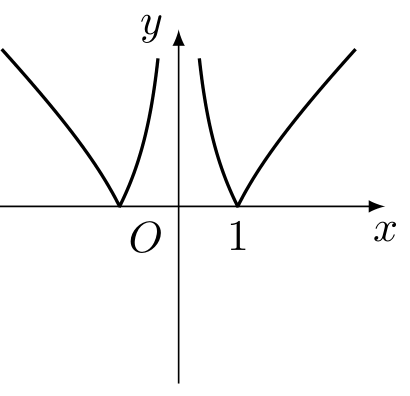
\includegraphics[width=0.15\paperwidth]{GaoKao/images/2022/tianjin/q3_option_c.png}\)  &  \(\text{D. }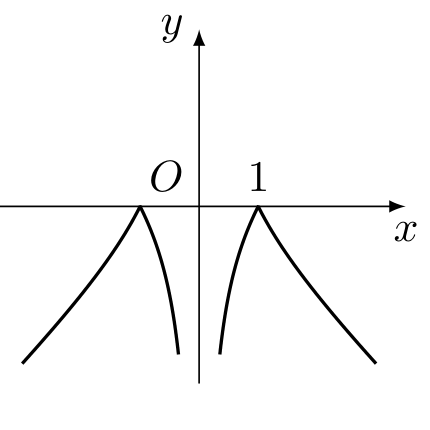
\includegraphics[width=0.15\paperwidth]{GaoKao/images/2022/tianjin/q3_option_d.png}\)
        \end{tabular*}
        \par}

        \item 为研究某药品的疗效，选取若干名志愿者进行临床试验，所有志愿者的舒张压数据（单位：kPa）的分组区间为 $[12,13),[13,14),[14,15),[15,16),[16,17]$，将其按从左到右的顺序分别编号为第一组，第二组，$\cdots$，第五组，如图是根据试验数据制成的频率分布直方图．已知第一组与第二组共有20人，第三组中没有疗效的有6人，则第三组中有疗效的人数为
        
        \textsf{[插入图片：频率分布直方图]}

        {\centering\begin{tabular*}{\linewidth}{@{}@{\extracolsep{\fill}}llll@{}}
          \(\text{A. }8\)  & \(\text{B. }12\)  & \(\text{C. }16\)  & \(\text{D. }18\)
        \end{tabular*}\par}

        \item 已知 $a=2^{0.7}$，$b=\bigl(\dfrac{1}{3}\bigr)^{0.7}$，$c=\log_2\dfrac{1}{3}$，则
       
        {\centering\begin{tabular*}{\linewidth}{@{}@{\extracolsep{\fill}}llll@{}}
          \(\text{A. }a>c>b\)  & \(\text{B. }b>c>a\)  & \(\text{C. }a>b>c\)  & \(\text{D. }c>a>b\)
        \end{tabular*}\par}

        \item 化简 $(2\log_4 3+\log_8 3)(\log_3 2+\log_9 2)$ 的值为
       
        {\centering\begin{tabular*}{\linewidth}{@{}@{\extracolsep{\fill}}llll@{}}
          \(\text{A. }1\)  & \(\text{B. }2\)  & \(\text{C. }4\)  & \(\text{D. }6\)
        \end{tabular*}\par}

        \item 已知抛物线 $y^2=4\sqrt{5}x$，$F_1,F_2$ 分别是双曲线 $\dfrac{x^2}{a^2}-\dfrac{y^2}{b^2}=1\,(a>0,b>0)$ 的左、右焦点，抛物线的准线过双曲线的左焦点 $F_1$，与双曲线的渐近线交于点 $A$，若 $\angle F_1F_2A=\dfrac{\pi}{4}$，则双曲线的标准方程是
       
        {\centering\begin{tabular*}{\linewidth}{@{}@{\extracolsep{\fill}}llll@{}}
          \(\text{A. }\dfrac{x^2}{10}-\dfrac{y^2}{4}=1\)  & \(\text{B. }x^2-\dfrac{y^2}{16}=1\)  & \(\text{C. }x^2-\dfrac{y^2}{4}=1\)  & \(\text{D. }\dfrac{x^2}{4}-\dfrac{y^2}{16}=1\)
        \end{tabular*}\par}

        \item 如图，"十字歇山"是由两个直三棱柱重叠后的景象，重叠后的底面为正方形．直三棱柱的底面是顶角为 $120^\circ$，腰为 $3$ 的等腰三角形，则该几何体的体积为
        
        {\centering
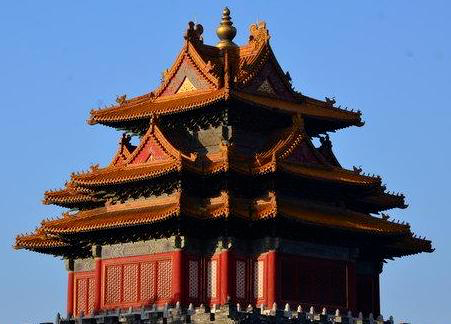
\includegraphics[width=0.65\linewidth]{GaoKao/images/2022/tianjin/q8_fig1.png}
\par}

        {\centering\begin{tabular*}{\linewidth}{@{}@{\extracolsep{\fill}}llll@{}}
          \(\text{A. }23\)  & \(\text{B. }24\)  & \(\text{C. }26\)  & \(\text{D. }27\)
        \end{tabular*}\par}

        \item 已知 $f(x)=\dfrac{1}{2}\sin2x$，关于该函数有下面四个说法：

        \ding{172}$f(x)$ 的最小正周期为 $2\pi$；
        \ding{173}$f(x)$ 在 $\bigl[-\dfrac{\pi}{4},\dfrac{\pi}{4}\bigr]$ 上单调递增；
        \ding{174}当 $x\in\bigl[-\dfrac{\pi}{6},\dfrac{\pi}{3}\bigr]$ 时，$f(x)$ 的取值范围为 $\bigl[-\dfrac{\sqrt{3}}{4},\dfrac{\sqrt{3}}{4}\bigr]$；
        \ding{175}$f(x)$ 的图象可由 $g(x)=\dfrac{1}{2}\sin\bigl(2x+\dfrac{\pi}{4}\bigr)$ 的图象向右平移 $\dfrac{\pi}{8}$ 个单位长度得到．

        以上四个说法中，正确的个数为
       
        {\centering\begin{tabular*}{\linewidth}{@{}@{\extracolsep{\fill}}llll@{}}
          \(\text{A. }1\)  & \(\text{B. }2\)  & \(\text{C. }3\)  & \(\text{D. }4\)
        \end{tabular*}\par}
    \end{enumerate}
\end{description}

\begin{description}
    \item[二、填空题] 本题共6小题，每小题5分，共30分．
    \begin{enumerate}[leftmargin=5pt]
      \addtocounter{enumi}{+9}
        \item 已知 $\i$ 是虚数单位，化简 $\dfrac{11-3\i}{1-2\i}$ 的结果为 \rule[-0.3ex]{3em}{0.4pt}．
        \item $\bigl(\sqrt{x}+\dfrac{3}{x^2}\bigr)^5$ 的展开式中的常数项为 \rule[-0.3ex]{3em}{0.4pt}．
        \item 若直线 $x-y+m=0\,(m>0)$ 与圆 $(x-1)^2+(y-1)^2=3$ 相交所得的弦长为 $m$，则 $m=$ \rule[-0.3ex]{3em}{0.4pt}．
        \item 已知 $x>0$，$y>0$，且 $x+2y=1$，则 $\dfrac{2y}{x}+\dfrac{x}{y}$ 的最小值为 \rule[-0.3ex]{3em}{0.4pt}．
        \item 52张扑克牌，没有大小王，无放回地抽取两次，则两次都抽到 $A$ 的概率为 \rule[-0.3ex]{3em}{0.4pt}；已知第一次抽到的是 $A$，则第二次抽到 $A$ 的概率为 \rule[-0.3ex]{3em}{0.4pt}．
        \item 在 $\triangle ABC$ 中，$\overrightarrow{CA}=\bm a$，$\overrightarrow{CB}=\bm b$，$D$ 是 $AC$ 的中点，$\overrightarrow{CB}=2\overrightarrow{BE}$，试用 $\bm a,\bm b$ 表示 $\overrightarrow{DE}$ 为 \rule[-0.3ex]{3em}{0.4pt}；若 $\overrightarrow{AB}\perp\overrightarrow{DE}$，则 $\angle ACB$ 的最大值为 \rule[-0.3ex]{3em}{0.4pt}．
    \end{enumerate}
\end{description}

\begin{description}
    \item[三、解答题] 本题共5小题，共75分．解答应写出文字说明、证明过程或演算步骤．
    \begin{enumerate}[leftmargin=5pt]
      \addtocounter{enumi}{+15}
        \item （14分）

        在 $\triangle ABC$ 中，角 $A,B,C$ 所对的边分别为 $a,b,c$．已知 $a=\sqrt{6}$，$b=2c$，$\cos A=-\dfrac{1}{4}$．

        \begin{enumerate}[label=(\arabic*)]
            \item 求 $c$ 的值；
            \item 求 $\sin B$ 的值；
            \item 求 $\sin(2A-B)$ 的值．
        \end{enumerate}

        \item （15分）

        如图，在直三棱柱 $ABC$-$A_1B_1C_1$ 中，$AB\perp AC$，$AB=AC=2$，$AA_1=4$，点 $D$ 是 $BC$ 的中点．

        {\centering
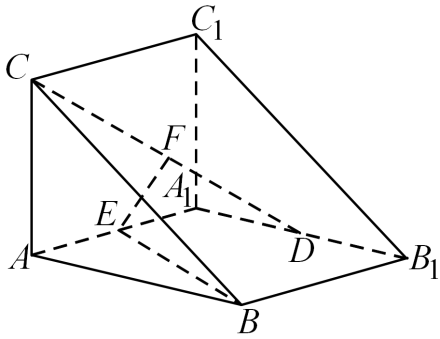
\includegraphics[width=5.3cm]{GaoKao/images/2022/tianjin/q17_fig1.png}
\par}

        \begin{enumerate}[label=(\arabic*)]
            \item 求异面直线 $A_1B$ 与 $C_1D$ 所成角的余弦值；
            \item 求平面 $ADC_1$ 与平面 $A_1DB$ 的夹角的正弦值．
        \end{enumerate}

        \item （15分）

        设 $\{a_n\}$ 为等差数列，$\{b_n\}$ 为等比数列，且 $a_1=b_1=a_2-b_2=a_3-b_3=1$．

        \begin{enumerate}[label=(\arabic*)]
            \item 求 $\{a_n\}$ 与 $\{b_n\}$ 的通项公式；
            \item 设 $\{a_n\}$ 的前 $n$ 项和为 $S_n$，求证：$(S_{n+1}+a_{n+1})b_n=S_{n+1}b_{n+1}-S_nb_n$；
            \item 求 $\displaystyle\sum_{k=1}^{2n}(-1)^k a_k b_{k}$．
        \end{enumerate}

        \item （15分）

        已知椭圆 $\dfrac{x^2}{a^2}+\dfrac{y^2}{b^2}=1\,(a>b>0)$ 的右焦点为 $F$，上顶点为 $B$，离心率为 $\dfrac{2\sqrt{5}}{5}$，且 $|BF|=\sqrt{5}$．

        \begin{enumerate}[label=(\arabic*)]
            \item 求椭圆的方程；
            \item 直线 $l$ 与椭圆有唯一的公共点 $M$，与 $y$ 轴的正半轴交于点 $N$，过 $N$ 与 $BF$ 垂直的直线交 $x$ 轴于点 $P$．若 $MP\parallel BF$，求直线 $l$ 的方程．
        \end{enumerate}

        \item （16分）

        已知 $a,b\in\mathbb{R}$，函数 $f(x)=\mathrm{e}^x-a\sin x$，$g(x)=b\sqrt{x}$．

        \begin{enumerate}[label=(\arabic*)]
            \item 求函数 $y=f(x)$ 在 $(0,f(0))$ 处的切线方程；
            \item 若 $y=f(x)$ 和 $y=g(x)$ 有公共点．
            \begin{enumerate}[label=(\roman*)]
                \item 当 $a=0$ 时，求 $b$ 的取值范围；
                \item 求证：$a^2+b^2>\mathrm{e}$．
            \end{enumerate}
        \end{enumerate}
    \end{enumerate}
\end{description}
\clearpage


\subsection{2022年浙江卷}\label{gk:2022年浙江卷}

\begin{description}
    \item[一、选择题] 本题共10小题，每小题4分，共40分．在每小题给出的四个选项中，只有一项是符合题目要求的．
    \begin{enumerate}[leftmargin=5pt]
        \item 设集合 $A=\{1,2,4,6\}$，$B=\{2,3,4,5\}$，则 $A\cap B=$
       
        {\centering\begin{tabular*}{\linewidth}{@{}@{\extracolsep{\fill}}llll@{}}
          \(\text{A. }\{2\}\)  & \(\text{B. }\{2,4\}\)  & \(\text{C. }\{2,4,6\}\)  & \(\text{D. }\{1,2,3,4,5,6\}\)
        \end{tabular*}\par}

        \item 已知 $a,b\in\mathbb{R}$，$a+3\i=(b+\i)\i$（$\i$ 为虚数单位），则
       
        {\centering\begin{tabular*}{\linewidth}{@{}@{\extracolsep{\fill}}llll@{}}
          \(\text{A. }a=1,b=-3\)  & \(\text{B. }a=-1,b=3\)  & \(\text{C. }a=-1,b=-3\)  & \(\text{D. }a=1,b=3\)
        \end{tabular*}\par}

        \item 若实数 $x,y$ 满足约束条件 $\begin{cases}x-2\geqslant0,\\2x+y-7\leqslant0,\\x-y-2\leqslant0,\end{cases}$ 则 $z=3x+4y$ 的最大值是
       
        {\centering\begin{tabular*}{\linewidth}{@{}@{\extracolsep{\fill}}llll@{}}
          \(\text{A. }20\)  & \(\text{B. }18\)  & \(\text{C. }16\)  & \(\text{D. }6\)
        \end{tabular*}\par}

        \item 设 $x\in\mathbb{R}$，则"$\sin x=1$"是"$\cos x=0$"的
       
        {\centering\begin{tabular*}{\linewidth}{@{}@{\extracolsep{\fill}}llll@{}}
          \(\text{A. }\)充分不必要条件  & \(\text{B. }\)必要不充分条件  & \(\text{C. }\)充要条件  & \(\text{D. }\)既不充分也不必要条件
        \end{tabular*}\par}

        \item 某几何体的三视图如图所示（单位：cm），则该几何体的体积（单位：$\text{cm}^3$）是
        
        {\centering
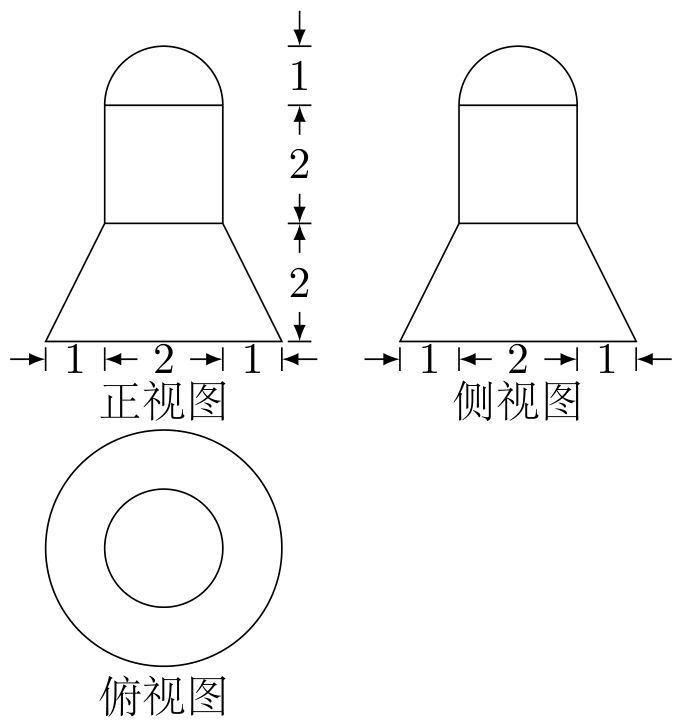
\includegraphics[width=6.7cm]{GaoKao/images/2022/zhejiang/q5_fig1.png}
\par}

        {\centering\begin{tabular*}{\linewidth}{@{}@{\extracolsep{\fill}}llll@{}}
          \(\text{A. }22\pi\)  & \(\text{B. }26\pi\)  & \(\text{C. }\dfrac{22\pi}{3}\)  & \(\text{D. }\dfrac{26\pi}{3}\)
        \end{tabular*}\par}

        \item 为了得到函数 $y=2\sin3x$ 的图象，只要把函数 $y=2\sin\bigl(3x+\dfrac{\pi}{5}\bigr)$ 图象上所有的点
       
        {\centering\begin{tabular*}{\linewidth}{@{}@{\extracolsep{\fill}}llll@{}}
          \(\text{A. }\)向左平移 $\dfrac{\pi}{5}$ 个单位  & \(\text{B. }\)向右平移 $\dfrac{\pi}{5}$ 个单位  & \(\text{C. }\)向左平移 $\dfrac{\pi}{15}$ 个单位  & \(\text{D. }\)向右平移 $\dfrac{\pi}{15}$ 个单位
        \end{tabular*}\par}

        \item 已知 $2^a=5$，$\log_8 3=b$，则 $4^{a-3b}=$
       
        {\centering\begin{tabular*}{\linewidth}{@{}@{\extracolsep{\fill}}llll@{}}
          \(\text{A. }25\)  & \(\text{B. }5\)  & \(\text{C. }\dfrac{25}{9}\)  & \(\text{D. }\dfrac{5}{3}\)
        \end{tabular*}\par}

        \item 如图，已知正三棱柱 $ABC$-$A_1B_1C_1$，$AC=AA_1$，$E,F$ 分别是棱 $BC,A_1C_1$ 上的点．记 $EF$ 与 $AA_1$ 所成的角为 $\alpha$，$EF$ 与平面 $ABC$ 所成的角为 $\beta$，二面角 $F$-$BC$-$A$ 的平面角为 $\gamma$，则
        
        {\centering
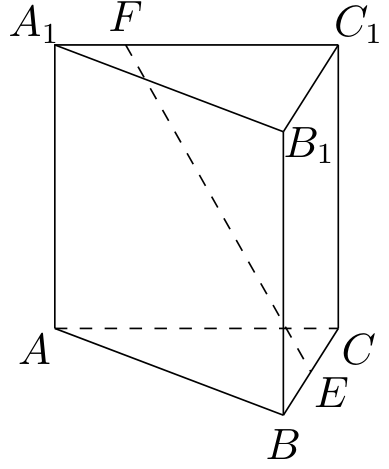
\includegraphics[width=4.5cm]{GaoKao/images/2022/zhejiang/q8_fig1.png}
\par}

        {\centering\begin{tabular*}{\linewidth}{@{}@{\extracolsep{\fill}}llll@{}}
          \(\text{A. }\alpha\leqslant\beta\leqslant\gamma\)  & \(\text{B. }\beta\leqslant\alpha\leqslant\gamma\)  & \(\text{C. }\beta\leqslant\gamma\leqslant\alpha\)  & \(\text{D. }\alpha\leqslant\gamma\leqslant\beta\)
        \end{tabular*}\par}

        \item 已知 $a,b\in\mathbb{R}$，若对任意 $x\in\mathbb{R}$，$a|x-b|+|x-4|-|2x-5|\geqslant0$，则
       
        {\centering\begin{tabular*}{\linewidth}{@{}@{\extracolsep{\fill}}llll@{}}
          \(\text{A. }a\leqslant1,b\geqslant3\)  & \(\text{B. }a\leqslant1,b\leqslant3\)  & \(\text{C. }a\geqslant1,b\geqslant3\)  & \(\text{D. }a\geqslant1,b\leqslant3\)
        \end{tabular*}\par}

        \item 已知数列 $\{a_n\}$ 满足 $a_1=1$，$a_{n+1}=a_n-\dfrac{1}{3}a_n^2\,(n\in\mathbb{N}^*)$，则
       
        {\centering\begin{tabular*}{\linewidth}{@{}@{\extracolsep{\fill}}llll@{}}
          \(\text{A. }2<100a_{100}<\dfrac{5}{2}\)  & \(\text{B. }\dfrac{5}{2}<100a_{100}<3\)  & \(\text{C. }3<100a_{100}<\dfrac{7}{2}\)  & \(\text{D. }\dfrac{7}{2}<100a_{100}<4\)
        \end{tabular*}\par}
    \end{enumerate}
\end{description}

\begin{description}
    \item[二、填空题] 本题共7小题，共36分．第11\textasciitilde14题每小题6分，第15\textasciitilde17题每小题4分．
    \begin{enumerate}[leftmargin=5pt]
      \addtocounter{enumi}{+10}
        \item 我国南宋著名数学家秦九韶，发现了从三角形三边求面积的"三斜求积"公式，即 $\triangle ABC$ 的三边分别为 $a,b,c$，则 $\triangle ABC$ 的面积 $S=\sqrt{\dfrac{1}{4}\Bigl[c^2a^2-\bigl(\dfrac{c^2+a^2-b^2}{2}\bigr)^2\Bigr]}$．若 $a=2$，$\sin C=\dfrac{\sqrt{3}}{2}$，$b+c=6$，则用"三斜求积"公式求得 $\triangle ABC$ 的面积为 \rule[-0.3ex]{3em}{0.4pt}，$\sin A=$ \rule[-0.3ex]{3em}{0.4pt}．
        \item 已知多项式 $(x+2)(x-1)^4=a_0+a_1x+a_2x^2+a_3x^3+a_4x^4+a_5x^5$，则 $a_2=$ \rule[-0.3ex]{3em}{0.4pt}，$a_1+a_2+a_3+a_4+a_5=$ \rule[-0.3ex]{3em}{0.4pt}．
        \item 若 $3\sin\alpha-\sin\beta=\sqrt{10}$，$\alpha+\beta=\dfrac{\pi}{2}$，则 $\sin\alpha=$ \rule[-0.3ex]{3em}{0.4pt}，$\cos2\beta=$ \rule[-0.3ex]{3em}{0.4pt}．
        \item 已知函数 $f(x)=\begin{cases}-x^2+2,&x\leqslant1,\\x+\dfrac{1}{x}-1,&x>1,\end{cases}$ 则 $f\bigl(f\bigl(\dfrac{1}{2}\bigr)\bigr)=$ \rule[-0.3ex]{3em}{0.4pt}；若当 $x\in[a,b]$ 时，$1\leqslant f(x)\leqslant3$，则 $b-a$ 的最大值为 \rule[-0.3ex]{3em}{0.4pt}．
        \item 现有7张卡片，分别写上数字 $1,2,2,3,4,5,6$．从这7张卡片中随机抽取3张，记所抽取卡片上数字的最小值为 $\xi$，则 $P(\xi=2)=$ \rule[-0.3ex]{3em}{0.4pt}，$E(\xi)=$ \rule[-0.3ex]{3em}{0.4pt}．
        \item 已知双曲线 $\dfrac{x^2}{a^2}-\dfrac{y^2}{b^2}=1\,(a>0,b>0)$ 的左焦点为 $F$，过 $F$ 且斜率为 $\dfrac{b}{4a}$ 的直线交双曲线于点 $A(x_1,y_1)$，交双曲线的渐近线于点 $B(x_2,y_2)$ 且 $x_1<0<x_2$．若 $|FB|=3|FA|$，则双曲线的离心率是 \rule[-0.3ex]{3em}{0.4pt}．
        \item 设点 $P$ 在单位圆的内接正八边形 $A_1A_2\cdots A_8$ 的边 $A_1A_2$ 上，则 $\overrightarrow{PA_1}^2+\overrightarrow{PA_2}^2+\cdots+\overrightarrow{PA_8}^2$ 的取值范围是 \rule[-0.3ex]{3em}{0.4pt}．
    \end{enumerate}
\end{description}

\begin{description}
    \item[三、解答题] 本题共5小题，共74分．解答应写出文字说明、证明过程或演算步骤．
    \begin{enumerate}[leftmargin=5pt]
      \addtocounter{enumi}{+17}
        \item （14分）

        在 $\triangle ABC$ 中，角 $A,B,C$ 所对的边分别为 $a,b,c$．已知 $4a=\sqrt{5}c$，$\cos C=\dfrac{3}{5}$．

        \begin{enumerate}[label=(\arabic*)]
            \item 求 $\sin A$ 的值；
            \item 若 $b=11$，求 $\triangle ABC$ 的面积．
        \end{enumerate}

        \item （15分）

        如图，已知 $ABCD$ 和 $CDEF$ 都是直角梯形，$AB\parallel DC$，$DC\parallel EF$，$AB=5$，$DC=3$，$EF=1$，$\angle BAD=\angle CDE=60^\circ$，二面角 $F$-$DC$-$B$ 的平面角为 $60^\circ$．设 $M,N$ 分别为 $AE,BC$ 的中点．

        {\centering
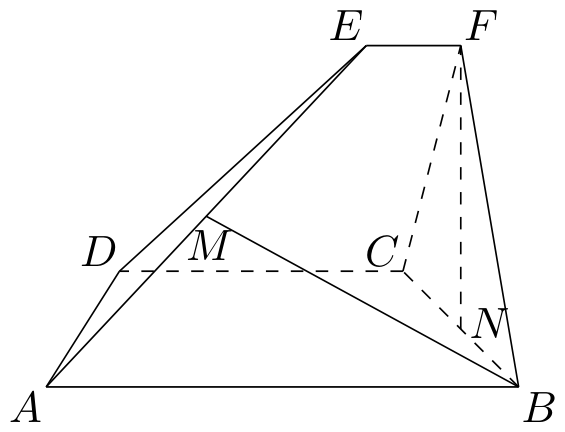
\includegraphics[width=9.8cm]{GaoKao/images/2022/zhejiang/q19_fig1.png}
\par}

        \begin{enumerate}[label=(\arabic*)]
            \item 证明：$FN\perp AD$；
            \item 求直线 $BM$ 与平面 $ADE$ 所成角的正弦值．
        \end{enumerate}

        \item （15分）

        已知等差数列 $\{a_n\}$ 的首项 $a_1=-1$，公差 $d>1$．记 $\{a_n\}$ 的前 $n$ 项和为 $S_n\,(n\in\mathbb{N}^*)$．

        \begin{enumerate}[label=(\arabic*)]
            \item 若 $S_4-2a_2a_3+6=0$，求 $S_n$；
            \item 若对于每个 $n\in\mathbb{N}^*$，存在实数 $c_n$，使 $a_n+c_n,a_{n+1}+4c_n,a_{n+2}+15c_n$ 成等比数列，求 $d$ 的取值范围．
        \end{enumerate}

        \item （15分）

        如图，已知椭圆 $\dfrac{x^2}{12}+y^2=1$．设 $A,B$ 是椭圆上异于 $P(0,1)$ 的两点，且点 $Q\bigl(0,\dfrac{1}{2}\bigr)$ 在线段 $AB$ 上，直线 $PA,PB$ 分别交直线 $y=-\dfrac{1}{2}x+3$ 于 $C,D$ 两点．

        {\centering
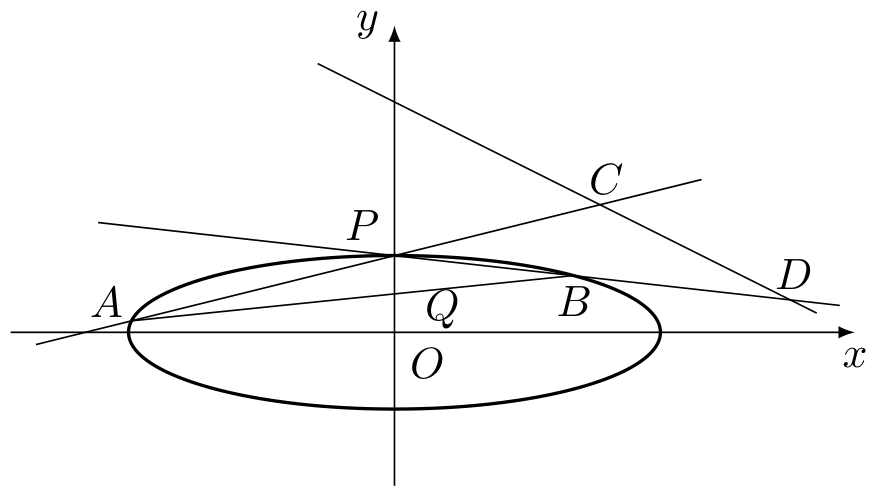
\includegraphics[width=4.5cm]{GaoKao/images/2022/zhejiang/q21_fig1.png}
\par}

        \begin{enumerate}[label=(\arabic*)]
            \item 求点 $P$ 到椭圆上点的距离的最大值；
            \item 求 $|CD|$ 的最小值．
        \end{enumerate}

        \item （15分）

        设函数 $f(x)=\dfrac{\mathrm{e}}{2x}+\ln x\,(x>0)$．

        \begin{enumerate}[label=(\arabic*)]
            \item 求 $f(x)$ 的单调区间；
            \item 已知 $a,b\in\mathbb{R}$，曲线 $y=f(x)$ 上不同的三点 $(x_1,f(x_1))$，$(x_2,f(x_2))$，$(x_3,f(x_3))$ 处的切线都经过点 $(a,b)$．证明：

            \begin{enumerate}[label=(\roman*)]
                \item 若 $a>\mathrm{e}$，则 $0<b-f(a)<\dfrac{1}{2}\bigl(\dfrac{a}{\mathrm{e}}-1\bigr)$；
                \item 若 $0<a<\mathrm{e}$，$x_1<x_2<x_3$，则 $\dfrac{2}{\mathrm{e}}+\dfrac{\mathrm{e}-a}{6\mathrm{e}^2}<\dfrac{1}{x_1}+\dfrac{1}{x_3}<\dfrac{2}{a}-\dfrac{\mathrm{e}-a}{6\mathrm{e}^2}$．
            \end{enumerate}
        \end{enumerate}
    \end{enumerate}
\end{description}
\clearpage


